\documentclass[12pt, a4paper]{article}
\usepackage [ngerman]{babel}
\usepackage[utf8]{inputenc}
\usepackage[T1]{fontenc}
%\renewcommand{\rmdefault}{phv} % Arial
%\renewcommand{\sfdefault}{phv} % Arial
\usepackage{color}
\usepackage{xcolor,colortbl}
\usepackage{fancyhdr}
\usepackage{fancybox}
\usepackage{graphicx}
\usepackage{geometry}
\usepackage{array}
\usepackage {ulem}
\usepackage{float}
\usepackage{eurosym}

\newcommand*{\textoverline}[1]{$\overline{\hbox{#1}}$}


\parindent0em

\geometry{verbose,a4paper,bmargin=30mm,lmargin=25mm,rmargin=20mm}


\pagestyle{fancy} %eigener Seitenstil
\fancyhf{} %alle Kopf- und Fußzeilenfelder bereinigen
\fancyhead[L]{Projekt BITS} %Kopfzeile links
\fancyhead[C]{\begin{tabular}{cc}
Stefan Schnürer & Benedikt Brüntrup\\Raphael Gregarek & Michael Dück
\end{tabular}} %zentrierte Kopfzeile
\fancyhead[R]{
\includegraphics[width=4cm]{Bilder/HS_OWL_RGB_Rot.jpg}} %Kopfzeile rechts
\renewcommand{\headrulewidth}{0.4pt} %obere Trennlinie
\fancyfoot[C]{\thepage} %Seitennummer
\renewcommand{\footrulewidth}{0.4pt} %untere Trennlinie
\usepackage{listings}

\setlength{\shadowsize}{1px}

%Quellcode-Darstellung #####################################
\definecolor{codeGray}{RGB}{240,240,240}
\definecolor{codeBlack}{RGB}{0,0,0}
\definecolor{codeRed}{RGB}{221,0,0}
\definecolor{codeBlue}{rgb}{0,0,187}
\definecolor{codeYellow}{RGB}{255,128,0}
\definecolor{CodeGreen}{rgb}{0.0,0.4,0.0}


\lstset{
  columns=fullflexible,
  showstringspaces=false,
  basicstyle= \normalsize,
  inputencoding=utf8,
  extendedchars=true,
}
\lstset{literate=%
{Ö}{{\"O}}1
{Ä}{{\"A}}1
{Ü}{{\"U}}1
{ß}{{\ss}}2
{ü}{{\"u}}1
{ä}{{\"a}}1
{ö}{{\"o}}1
{§}{{\S}}1
{_}{{\_}}1
}

\lstset
{
	backgroundcolor={\color{codeGray}},% 
    basicstyle={\small\ttfamily\color{codeBlack}},% 
    commentstyle={\color{CodeGreen}},%
    keywordstyle={\color{codeBlue}},%
    stringstyle={\color{codeRed}},%
    identifierstyle={\color{codeBlue}},%
    %
    % Zeilenumbrüche aktivieren, Leerzeichen nicht hervorheben
    breaklines=true,%
    showstringspaces=false,%
    % 
    % Listing-Caption unterhalb (bottom)
    captionpos=b,%
    frame=single,
    numbers=left, 
	numberstyle=\scriptsize,
	xleftmargin=2em
}

\renewcommand{\lstlistingname}{Quellcode}

\lstdefinelanguage{JavaScript} {
	morekeywords={
		break,const,continue,delete,do,while,export,for,in,function,
		if,else,import,in,instanceOf,label,let,new,return,switch,this,
		throw,try,catch,typeof,var,void,with,yield
	},
	sensitive=false,
	morecomment=[l]{//},
	morecomment=[s]{/*}{*/},
	morestring=[b]",
	morestring=[d]'
}

\lstdefinelanguage{CSS}
{
  morecomment=[s]{/*}{*/},
  keywords={visibility},
  morestring=[s]{\{}{\}},
}

\lstdefinelanguage{phpHtml}{
	 language=html,
	 alsolanguage=PHP,
	 alsolanguage=CSS,
	 alsolanguage=JavaScript
}




%###########################################


%Links im Inhaltsverzeichnis
\usepackage{hyperref}
\hypersetup{
    colorlinks,
    citecolor=black,
    filecolor=black,
    linkcolor=black,
    urlcolor=black
}


%###############################################

%Definition von Sonderzeichen
\DeclareUnicodeCharacter{20AC}{\euro}


% Verbesserung der Silbentrennung
\hyphenation{Sys-tem Sys-tem-en Java-Script}


\begin{document}

% ######################## Titelseite ######################## %

\begin{titlepage}
Hochschule Ostwestfalen-Lippe \\
Fachbereich 8 - Umweltingeneurwesen und Angewandte Informatik \\
Fachgebiet Angewandte Informatik \\
Projekt Realisierung betrieblicher IT-Systeme \\
4. Semester SoSe 2015\\
\vspace{2cm}

\begin{center}
\begin{Large}
\textbf{Ausarbeitung: \\Projekt Realisierung betrieblicher IT-Systeme } \\
\end{Large}
\vspace{2cm}

\begin{Large}
\textbf {Entwicklung eines Webshops\\ für das Fahrradproduktions- und Vertriebsunternehmen Global Bike Inc.} \\[0.35cm]
\end{Large}
\vspace{5mm}
Von \\[0.25cm]
Stefan Schnürer,\\[0.25cm]
Benedikt Brüntrup,\\[0.25cm]
Raphael Gregarek und\\[0.25cm]
Michael Dück
\end{center}

\vfill
Erstprüfer: Prof. Dr. rer. nat. Stefan Wolf\\
Zweitprüfer: Prof. Dr. Ralf Hesse\\
Drittprüfer: Prof. Dr. Jessica Rubart\\
Vierprüfer: Prof. Dr. rer. nat. Burkhard Wrenger\\[0.25cm]
Eingereicht am: \today
\end{titlepage}

% ######################## Dokument ######################## %

\hspace{1pt}
% ### Inhaltsverzeichnis ### %
\tableofcontents
\vfill


%Projektplanung
\newpage
\section{Projektaufgabenstellung$^1$}
Die Aufgabenstellung des Projekts ist es einen Webshop für die Firma Global Bike Inc. (folgend GBI) zu erstellen. Diese Firma stellt Fahrräder her und vermarktet diese. Die Produkte des Webshops sollen aus einem ERP-System geladen werden. Bei dem ERP-System handelt es sich um ein schon bestehendes SAP-ERP-System. Alle auf dem Webshop getätigten Bestellungen sollen an das ERP-System weitergereicht werden. Zudem soll für den Benutzer des Webshops der Stand der Bestellung einsehbar sein. Dieser Stand soll ebenfalls aus dem ERP-System übernommen werden. \\
Weitere Kriterien für den Webshop sind, dass dieser in eine APP für mobile Geräte einbindbar sein muss, ein Corporate-Design entworfen werden, sowie ein Marketing-Mix für die Online-Vermarktung im Großraum OWL entwickelt werden soll.

\section{Projektplanung}
Dieser Abschnitt erläutert, wie die Projektplanung dieses Projekts ablief. Es wird der Ablauf, von der Ideenfindung bis zur Planung der Durchführung, erläutert.

\subsection{Ideenfindung$^1$}
Der erste Schritt des Projekts bestand darin zu bestimmen, was für Funktionen der Webshop alles anbieten soll. Hierfür sind drei Onlinewebshops betrachtet worden. Es wurden die Webshops \glqq fahrrad.de\grqq{}, \glqq amazon.de\grqq{} und \glqq alternate.de\grqq{} angeschaut.\\
Vom Webshop \glqq alternate.de\grqq{} ist der Webseitenkopf als sehr sinnvoll empfunden worden. Dieser Kopf ist am oberen Rand der Webseite fest fixiert und wird nicht mitgescrollt. Dieses bietet den Vorteil, dass der Kunde durchgehend die Menge einsehen kann, die sich im Warenkorb befindet. Grund hierfür ist, dass sich eine kleine Warenkorbanzeige mit im Kopf der Webseite befindet. Zudem kann der Benutzer sich durch die Webseite navigieren ohne zu scrollen. Da ebenso im Kopf der Webseite die Suche fixiert ist, kann der Benutzer auch ohne zu scrollen nach etwas suchen. Wegen den vielen Vorteilen wurde beschlossen den Kopf der Webseite weitgehend für den Webshop der GBI zu übernehmen.\\
Aus allen drei Webshops wurde zudem übernommen, dass der Webshop der GBI mit einen Warenkorb gelöst werden soll und die Benutzer sollen Kommentare zu einen Artikel schreiben und lesen können. Ebenso soll es möglich sein, dass der Kunde den Artikel bewerten kann. Der Artikel soll über eine Suche und eine Navigation zugreifbar sein. Zu einen Artikel soll in der Produktbeschreibung mehrere Produktbilder angezeigt werden, die sich der Kunde durch draufklicken größer ansehen kann. Die Produktbeschreibungsseite soll mindestens den Preis, die Bewertung, den Produktnamen und eine ausführlichen Beschreibungstext erhalten.\\
Als negativ wurde empfunden, wenn die Startseite der Webseite \glqq überladen\grqq{} von Produkten ist. Somit wurde beschlossen die Startseite des Webshops übersichtlich zu gestalten.

\newpage
\subsection{Anforderungsanalyse$^2$}
Der zweite Schritt des Projekts war die Anforderungsanalyse. Hier wurde ermittelt, welche Anforderungen genau der Webshop erfüllen muss. Während der Analyse einigte man sich auf folgende Projektanforderungen:
\begin{itemize}
	\item Man sollte sich registrieren können.
	\item Wenn man schon registriert ist, sollte man sich anmelden können.
	\item Die Daten zwischen dem ERP-System und dem Webshop sollen über eine Schnittstellendatenbank ausgetauscht werden.
	\item Um auf mobilen Geräten und Desktop-Computern die Webseite richtig anzeigen zu können soll eine zusätzliche CSS-Datei für mobile Geräte erstellt werden. Diese Datei soll die Style-Anweisungen überschreiben, die vom mobilen Gerät falsch angezeigt werden.
	\item Man sollte ein Artikel über die Navigation und die Suche erreichen.
	\item Die gefundenen Artikel sollten in einen Warenkorb gesammelt werden können (mit Mengenangabe).
	\item Nachdem der Warenkorb gefüllt ist, sollen die Artikel bestellt werden können. Hierbei sollen verschiedene Liefer- und Zahlungsmöglichkeiten auswählbar sein.
	\item Die Bestellung sollte mit einer Bestätigungs-Email bestätigt werden.
	\item Der Zustand der Bestellung sollte nachverfolgbar sein.
	\item Der Kunde sollte den Artikel bewerten können und Kommentare äußern können.
\end{itemize}

\subsection{Geschäftsprozess$^1$}
Als nächstes wurde festgelegt, wie ein Geschäftsprozess beim Webshop aussehen soll. Der Geschäftsprozess beginnt, wenn der Kunde die Webseite aufruft. Darauf folgend registriert sich entweder der Kunde oder er loggt sich mit der vorhandenen Benutzerkennung ein. Danach sucht sich der Kunde Produkte auf der Webseite aus und füllt damit den Warenkorb. Nachdem der Warenkorb gefüllt ist, führt der Kunde die Bestellung durch. Wenn die Firma GBI die  Bestellung erhalten hat, wird an den Kunden eine Bestätigungsmail versendet. Darauf folgend wartet der Webshop auf die Bezahlung der Produkte. Hat die Firma GBI die Zahlung erhalten,  wird die Ware an den Kunden verschickt. \\Dieser Geschäftsprozess ist nochmal in dem als \glqq Business Process Model and Notation\grqq{} dargestellten Geschäftsmodell (\textit{Abbildung 1}) zu sehen.

\begin{figure}[H] 
  \centering
     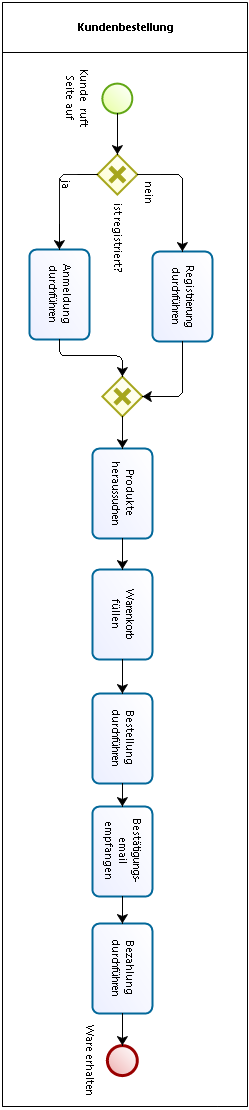
\includegraphics[width=50mm]{Bilder/Abbildung1-Geschaeftsprozess.png}
  \caption{Geschäftsprozess des Webshops}
  \label{fig:Abbildung 1}
\end{figure}


\subsection{Risikoanalyse$^2$}

Ein wichtiger Bestandteil der Projektplanung ist die Risikoanalyse. Sie umfasst alle ermittelten Risiken, die zur Laufzeit des Projekts auftreten können und entsprechende Gegenmaßnahmen. Um die Risiken zu ermitteln wurde zuvor eine Risikoanalyse durchgeführt. Bei der Risikoanalyse werden die Risiken hinsichtlich ihrer Tragweite und Wahrscheinlichkeit bewertet. Die Bewertung reicht dabei von gering, über eher gering, eher hoch bis hoch. \textit{Abbildung 2} zeigt die Einstufungen der Risiken zum Projekt sowie entsprechende Gegenmaßnahmen:

\begin{figure}[H] 
  \centering
     \fbox {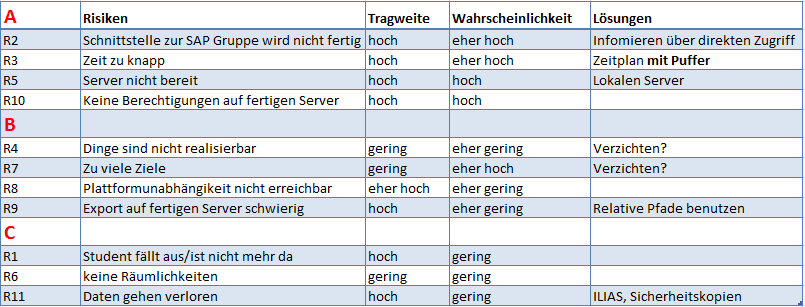
\includegraphics[width=15cm]{Bilder/Risikoanalyse1.png}}
  \caption{Einstufung der Risiken und entsprechende Gegenmaßnahmen}
  \label{fig:Abbildung 2}
\end{figure}

Die Risiken werden in drei Kategorien unterteilt. Kategorie A beschreibt Risiken, die eine hohe Tragweite und Wahrscheinlichkeit aufweisen. Kategorie B beschreibt Risiken, deren Tragweite und Wahrscheinlichkeit weder zu hoch noch zu gering eingestuft wurden. Kategorie C beschreibt Risiken, deren Tragweite und Wahrscheinlichkeit eher gering eingestuft wurden.

Der Kategorie A wurden die Risiken „SAP-Gruppe wird nicht mit Datenbank fertig“, „Zeit zu knapp“, „Server nicht bereit“ und „Keine Berechtigungen auf fertigen Server“ hinzugefügt.  Das Risiko des Zeitmangels ist bei den meisten Projekten das größte Problem. Mangelnde Zeit bedeutet, dass das Projekt nicht im vollen Umfang fertiggestellt werden kann. Daher wurde es als eines der höchsten Risiken eingestuft. Risiken im Zusammenhang mit dem Server fallen ebenfalls unter dieser Kategorie. Ohne einen Server kann die Seite nicht betrieben werden, weshalb dieser kontinuierlich zur Verfügung stehen muss. Die SAP-Gruppe ist die wichtigste Schnittstelle, die es zu beachten gilt, da diese die Datenbank für den Webshop zur Verfügung stellt. Ohne Datenbank ist der Webshop nicht voll funktionsfähig.
\\
Der Kategorie B wurden die Risiken „Dinge sind nicht realisierbar“, „Zu viele Ziele“, „Plattformunabhängigkeit nicht erreichbar“ und „Export auf fertigen Server schwierig“ hinzugefügt. Wenn sich bei den Zielen eines Projekts verschätzt wird und dadurch zu viele oder unrealistische Ziele gesetzt werden, kann nicht der vorher vereinbarte Umfang des Projekts gewährleistet werden. Plattformunabhängigkeit ist eines der vereinbarten Anforderungen. Der Webshop sollte auf jeden Browser dargestellt werden können. Je mehr Browser die Webseite unterstützt, desto mehr Kunden können angesprochen werden. Der Export auf den fertigen Server könnte sich als schwierig erweisen, wenn Programme, die für den Export benötigt werden, nicht auf dem Server vorhanden sind.
\\
Der Kategorie C wurden die Risiken „Student fällt aus/ist nicht mehr da“, „keine Räumlichkeiten vorhanden“ und „Daten gehen verloren“ hinzugefügt. Diese Risiken können auftreten, sind aber für das Projekt keine große Bedrohung. Das Risiko eines Datenverlustes wird durch mehrere Backups stark gemindert.
\\
Das Risiko „Student fällt aus/ist nicht mehr da“ wurde anfangs als gering eingestuft.  Zum jetzigen Zeitpunkt wird dieses Risiko allerdings als hoch eingestuft, da die Gruppenmitglieder Herr Gregarek und Herr Dück schon mehrfach ausgefallen sind.
\\
\textit{Abbildung 3} zeigt die Ergebnisse der Risikoanalyse anhand einer Grafik:

\begin{figure}[H] 
  \centering
     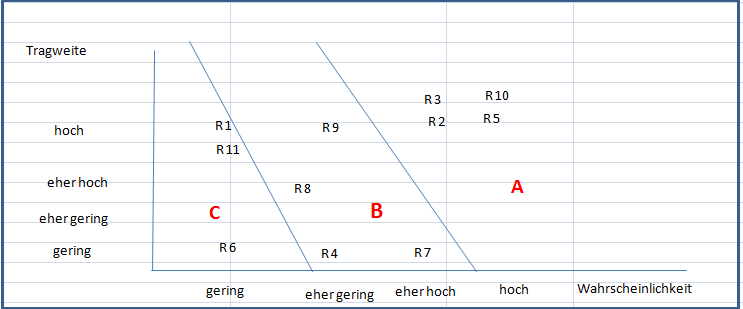
\includegraphics[width=15cm]{Bilder/Risikoanalyse2.png}
  \caption{Ergebnisse der Risikoanalyse}
  \label{fig:Abbildung 3}
\end{figure}

Dabei lässt sich die Einteilung der Risiken in den einzelnen Kategorien besser nachvollziehen.

\subsection{Wahl der Programmiersprache$^1$}
Nachdem die Anforderungen an das Projekt festgelegt waren, wurde sich mit der Festlegung der Programmiersprache beschäftigt. Es stand Java Enterprise Edition und PHP zur Auswahl. Die Auswahl fiel auf PHP, da aus alten Projekten und der Webdesign-Vorlesung schon Vorwissen über die Programmierung von Webseiten in PHP vorhanden war. Zudem war auch geplant Teile des Quellcodes der alten Projekte für das neue Projekt wieder zu verwenden.

\subsection{Wahl der Programmierentwicklungsumgebung und des Versions-verwaltungs-Plugin$^1$}
Zu Beginn des Projekts hatte jedes Gruppenmitglied einen eigenen Texteditor und an einer eigenen Version des Projekts gearbeitet. Es fiel nach kurzer Zeit auf, dass so das Zusammenfügen der verschiedenen Versionen sehr aufwendig war. Aus diesen Grund wurde nach einer Möglichkeit gesucht, das Problem zu lösen. Es wurde das \glqq GitHub-Plugin\grqq{} für das Programm \glqq Eclipse\grqq{} als Lösung für das Versionsproblem gefunden. \\
Als Entwicklungsumgebung wurde sich für Eclipse entschlossen, da es bei installierten PHP-Plugin eine gute Autovervollständigung für PHP bietet. Zudem ist es als Portable-Version erhältlich und kann somit ohne Installation auf den Hochschulrechnern betrieben werden. \\
Als Versionsverwaltungssystem wurde sich für \glqq GitHub\grqq{} entschlossen, da dieses schon in den Programm \glqq Eclipse\grqq{} integriert ist. Zudem ist „GitHub“ eine Cloud basierte Lösung, welche das gemeinsame Arbeiten an einen Projekt ermöglicht. Das komplette Projekt wird dabei auf einen Server hochgeladen. Jedes Gruppenmitglied, das einen Account bei „GitHub“ erstellt hat, kann dem Projekt beitreten, indem es bei den Gruppen-Administrator um Erlaubnis bittet. Dadurch kann ein Dokument von mehreren Gruppenmitgliedern gemeinsam bearbeitet werden. So entstehen mehrere Versionen von einem Dokument, die anschließend wieder mit Hilfe eines in GitHub enthaltenden \glqq Merge-Tools\grqq{} zu einer gemeinsamen Version zusammengefügt werden können.


\subsection{Grundlegender Aufbau und Ordnerstruktur der Webseite$^1$}
Einer der ersten Schritte der praktischen Umsetzung des Projekts war die Festlegung der Ordnerstruktur der Webseite. Die Ordnerstruktur sollte einen einheitlichen Aufbau der Webseite garantieren. Mit der Festlegung sollte für jedes Projektmitglied definiert werden, wo welche Dateien abgelegt werden sollen und wie generell die programmiertechnische Struktur des Programms aussehen soll.  \\
Als Programmieransatz für das Projekt wurde die objektorientierte Programmierung gewählt. Die Hauptgründe für die Auswahl des Programmieransatzes waren, dass die objektorientierte Programmierung durch die Vererbung die Möglichkeit bietet schon programmierte Funktionen an andere Klassen zu übernehmen. Es wird also Programmierarbeit eingespart. Ein Beispiel für die Einsparung von Programmierarbeit ist, wenn ein Fehler in einer vererbten Methode ist, muss der Fehler nur bei der Eltern-Klasse behoben werden und nicht bei der Kind-Klasse. Ein weiterer Grund ist, dass die objektorientierte Programmierung auch die Übersichtlichkeit der Webseite fördert. Für jedes Objekt der Webseite wird einfach eine Klasse angelegt, welche dieses definiert. So wird z.B. eine Klasse für den Kunden oder den Warenkorb erstellt. Diese Klasse arbeitet alle Aufgaben des Objekts ab. Der letzte Grund für den Ansatz war, dass schon objektorientierte Quellcodes aus alten Projekten zur Verfügung standen. \\
Da sich für die objektorientierte Programmierung entschieden wurde, hat sich die Gruppe auf folgende Ordnerstruktur geeinigt:
\begin{figure}[H]
  \centering
     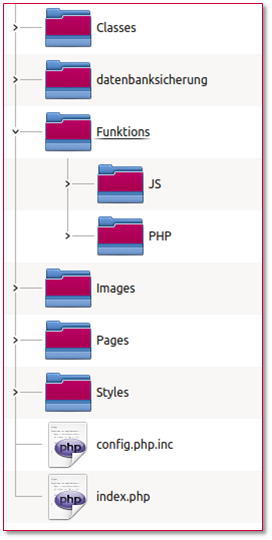
\includegraphics[width=45mm]{Bilder/ordnerstruktur.png}
  \caption{Ordnerstruktur des Projekts}
  \label{fig:Abbildung 4}
\end{figure}
Der Ordner \glqq Classes\grqq{} beinhaltet alle PHP-Klassen des Projekts. Dieser Ordner enthält zum Beispiel Klassen zur Umsetzung des Warenkorbs, des Datenbankzugriffs, des Kundens, der Kundenbestellung und so weiter. Der Ordner \glqq datenbanksicherung\grqq{} enthält die jeweils aktuelle Sicherung der Datenbank. Der folgende Ordner ist in zwei Unterordner aufgeteilt. Dieser Ordner wurde mit dem Namen \glqq Funktions\grqq{} bezeichnet. Der erste Unterordner, der den Namen \glqq JS\grqq{} trägt, enthält die clientseitig programmierten Funktionen. Die clientseitige Programmierung sollte in JavaScript umgesetzt werden. Aus diesen Grund sind in diesen Ordner JavaScript-Dateien vorzufinden. Die JavaScripts werden unter anderen dafür verwendet eine Formulareingabe vor den Absenden auf Gültigkeit zu überprüfen. Dieses sorgt dafür, dass es nicht zu unnötigen Datenverkehr zwischen Browser und Webserver kommt. Der Unterordner \glqq PHP\grqq{} enthält die Funktionen, die zum Beispiel nach dem Absenden einer Formulareingabe an den Webserver aufgerufen werden. Diese Funktionen instanzieren die Klassen. Zudem rufen die Funktionen-Dateien die entsprechenden Methoden auf, um die vom Formular empfangenen Eingaben zu verarbeiten. Dieser Ordner enthält noch zwei weitere Dateien. Die erste der beiden Dateien heißt \glqq set\_page.php.inc\grqq{}. Diese Datei ließt einen über die Adressenzeile erhaltenden Parameter aus. Anhand des Parameters bestimmt die Datei, welcher Inhalt aktuell auf der Webseite angezeigt werden soll. Hierzu inkludiert die Datei die entsprechende HTML-Seite aus dem Ordner \glqq Pages\grqq{}. Die zweite Datei heißt \glqq  set\_control.php.inc\grqq{}. Diese Datei inkludiert die benötigte Funktions-Datei, die z.B. die Formulareingaben bearbeiten. \\
In diesem Projekt werden keine in PHP programmierten Funktionen und Inhaltseiten direkt aufgerufen. Diese Dateien werden immer in die Index.php inkludiert. Der Grund hierfür ist, dass so dem Anwender der interne Aufbau der Webseite verborgen bleibt.\\
Der Ordner \glqq Images\grqq{} enthält die Bilder, die auf der Webseite angezeigt werden. Der letzte Ordner mit dem Namen \glqq Styles\grqq{} enthält die CSS-Dateien, die das Design der Webseite festlegen. In der \glqq config.php.inc\grqq{}-Datei werden grundlegende Konfigurationen für den Webshop festgelegt. In dieser Datei sind unter anderen die Zugangsdaten für die Datenbank angegeben. Die \glqq index.php\grqq{} ist die standardmäßige Webseiteneinstiegsdatei. Über diese Datei wird die Webseite geladen.

\subsection{Die Test-Server$^1$}
Um bei der Entwicklung nicht erst darauf warten zu müssen bis die Server-Gruppe die benötigten Server-Dienst aufgesetzt hat, wurde sich nach eine Möglichkeit umgesehen, wie man für Testzwecke die Webseite auf den Hochschulrechnern laufen lassen könnte. Hierfür wurde das Programm XAMPP gefunden. Es ist eine Software-Sammlung, die alle benötigten Server-Dienste für PHP-Webseiten auf einen Windows-Rechner bereitstellt. Die Softwaresammlung bietet den Vorteil, dass eine portable Version erhältlich ist. Diese Version kann ohne Administrationsrechte ausgeführt werden.

\subsection{Zeitplan$^2$}
Nachfolgend wird der Zeitplan des Projekts dargestellt. Für jedes Arbeitspaket wurde eine Zeit von zwei Wochen eingeplant. Da jedes Gruppenmitglied 3 Arbeitspakte zugeteilt bekam, betrug die reine Arbeitszeit 6 Wochen. Herr Schnürer und Herr Brüntrup konnte diese Zeit weitestgehend einhalten. Zu der Arbeitszeit von Herrn Gregarek und Herrn Dück  ist nichts Näheres bekannt. Da deren Arbeitspakte jedoch nicht vollständig bearbeitet wurden, ist deren Arbeitszeit deutlich geringer einzuschätzen. Die Arbeitszeit von 6 Wochen trug dazu bei, dass die Sommersemesterferien als Pufferzeit eingeplant werden konnten. \textit{Abbildung 5} zeigt den Zeitplan, während \textit{Abbildung 6} das dazugehörige Gantt-Diagramm zeigt. \textit{Abbildung 7-10} beschreiben den aktuellen Projektstand vom 07. August 2015 anhand eines Ampelsystems. 

\begin{figure}[H] 
  \centering
     \fbox{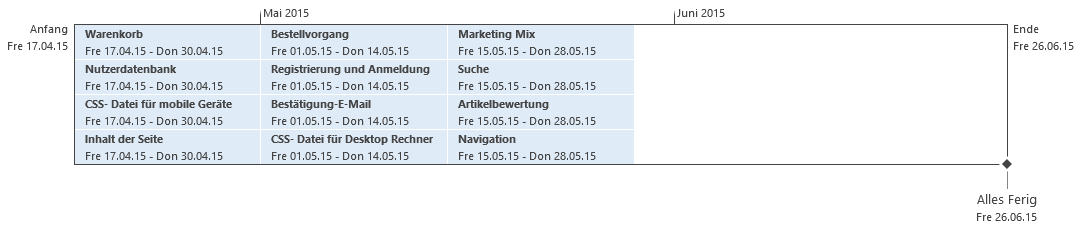
\includegraphics[width=160mm]{Bilder/Abbildung16_Zeitplan.png}}
  \caption{Zeitplan}
\end{figure}

\begin{figure}[H] 
  \centering
     \fbox{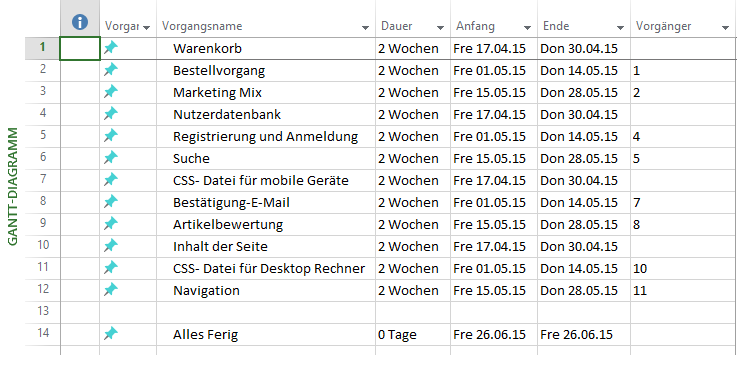
\includegraphics[width=15cm]{Bilder/Abbildung17_GanttDiagramm.png}}
  \caption{Zeitplan}
\end{figure}

\begin{figure}[H] 
  \centering
  \fbox{
     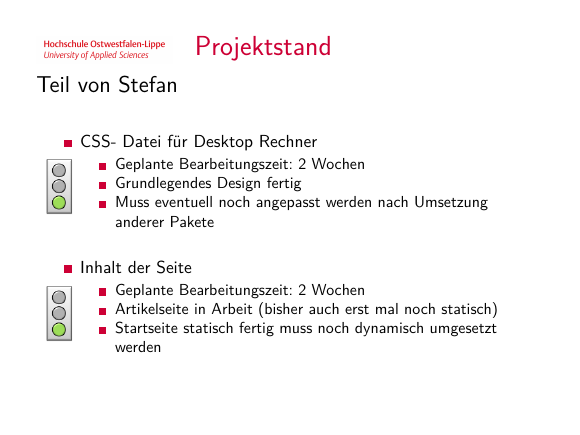
\includegraphics[width=10cm]{Bilder/projektstand1.png}}
  \caption{Zeitplan}
\end{figure}


\begin{figure}[H] 
  \centering
  \fbox{
     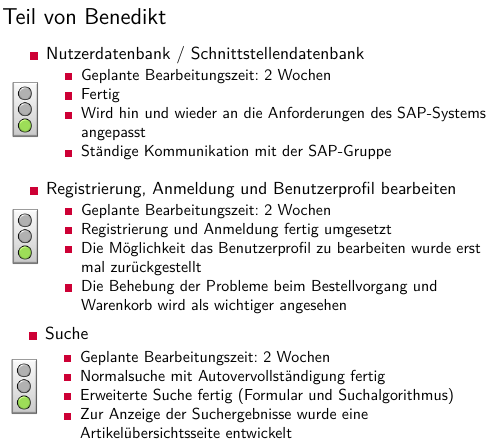
\includegraphics[width=10cm]{Bilder/projektstand3.png}}
  \caption{Zeitplan}
\end{figure}


\begin{figure}[H] 
  \centering
  \fbox{
     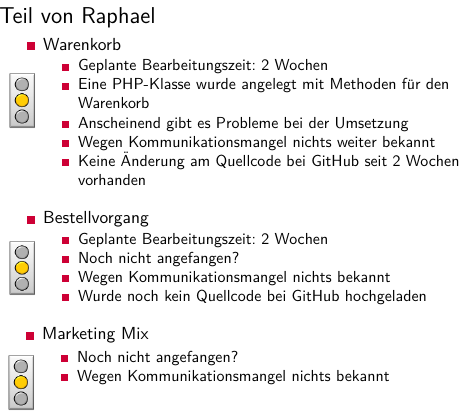
\includegraphics[width=10cm]{Bilder/projektstand5.png}}
  \caption{Zeitplan}
\end{figure}


\begin{figure}[H] 
  \centering
  \fbox{
     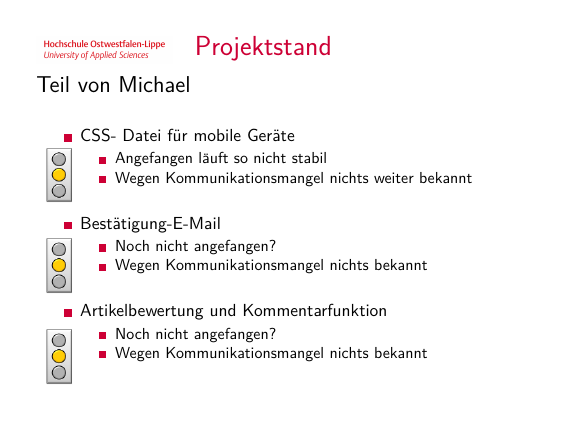
\includegraphics[width=10cm]{Bilder/projektstand7.png}}
  \caption{Zeitplan}
\end{figure}



%Realisierung
\section{Arbeitspakete}
Dieser Abschnitt beschreibt die Unterteilung des Projektes in Arbeitspakete und wie die Gruppenmitglieder die zugeteilten Arbeitspakte abarbeitet haben. Es wird auch auf den unvorhergesehenen Arbeitsbereitschaftsmangel der Gruppenmitglieder Herr Gregarek und Herr Dück eingegangen.

\subsection{Einteilung der Arbeitspakete}
Zunächst wurden die Arbeitspakete aus der Anforderungsanalyse abgeleitet. Aus dieser Ableitung sind folgende Arbeitspakete definiert worden:
\begin{enumerate}
	\item Entwicklung des grundlegenden Webseitendesigns für Desktop-Rechner
	\item Anpassung des Designs für mobile Geräte
	\item Entwicklung der Webseitennavigationsleiste
	\item Entwicklung der inhaltlichen Seiten des Webshops:
	\begin{itemize}
		\item Startseite
		\item Produktseite
		\item Rechtliche Seiten:
		\begin{itemize}
			\item[$\diamond$] Impressum
			\item[$\diamond$] Datenschutz
			\item[$\diamond$] AGB
		\end{itemize}
	\end{itemize}
	\item Entwicklung einer Schnittstellendatenbank zum Datenaustausch zwischen Webshop und SAP-System:
	\begin{itemize}
		\item Ansprechpartner der SAP-Gruppe für die Schnittstelle zum Webshop
		\item Entwurf von Tabellen für die Datenhaltung des Webshops 
	\end{itemize}
	\item Registrierungs- und Anmeldungsfenster designen und programmieren
	\begin{itemize}
		\item Möglichkeit den Kunden bieten die Anmeldeinformationen später verändern zu können
	\end{itemize}
	\item Entwickeln einer Suchfunktion:
	\begin{itemize}
		\item Autovervollständigung
		\item Erweiterte Suchfunktion, wo die Suche genauer eingegrenzt werden kann
		\item Auflistung der Suchergebnisse
	\end{itemize}
	\item Warenkorb
	\begin{itemize}
		\item Auflistung der Produkte, die sich im Warenkorb befinden
		\item Formular mit Mengenfeld, um ein Produkt in den Warenkorb zu packen
		\item Möglichkeit zur nachträglichen Änderung der Produkte im Warenkorb:
		\begin{itemize}
			\item[$\diamond$] Änderung der Bestellmenge
			\item[$\diamond$] Entfernen des Produkts aus dem Warenkorb
		\end{itemize}
	\end{itemize}
	\item Bestellvorgang:
	\begin{itemize}
		\item Bestellroutine mit folgenden Schritten:
		\begin{itemize}
			\item[$\diamond$] Wahl der Versandart
			\item[$\diamond$] Nachträglichen Änderung der Bestellmenge der Produkte
			\item[$\diamond$] Wahl Zahlungsart
			\item[$\diamond$] Wahl Lieferadresse
			\item[$\diamond$] Bestellübersichtseite zur Kontrolle vor den Absenden der Bestellung
		\end{itemize}
		\item Einsicht des aktuellen Status der Bestellung
		\item Möglichkeit die Bestellung zu stornieren
	\end{itemize}
	
	\item Erstellung eines Marketing Mix
	\item Bewertungsfunktion von Artikel (mit Kommentarfunktion)
	\item Email-Versand
	\begin{itemize}
		\item Klasse für den Email-Versand entwerfen
		\item Designen der Bestätigungs-Emails
	\end{itemize}					 
\end{enumerate}

Die oben genannten Arbeitspakete hat sich die Gruppe untereinander aufgeteilt. Stefan Schnürer hat Arbeitspakete 1,3 und 4 übernommen. Benedikt Brüntrup übernahm die Arbeitspakete 5, 6 und 7. Michael Dück hatte sich bereit erklärt die Arbeitspakte 2, 11 und 12 zu bearbeiten. Raphael wollte die Arbeitspakete 8, 9 und 10 abarbeiten.


%Nachfolgend soll auf die einzelnen Zwischenschritte des Projektes eingegangen werden.Das Projekt beginnt mit der Projektplanung. Hierbei werden die Arbeitspakete definiert und an den entsprechenden Gruppenmitgliedern verteilt. Pro Arbeitspaket wird eine Bearbeitungsdauer von zwei Wochen festgelegt. Es wird ein Projektzeitplan sowie eine Risikoanalyse erstellt. Im Anschluss daran werden grobe Design Entwürfe für die Homepage erstellt. Es wird sich für den Design Entwurf von Herrn Brüntrup entschieden. Die Homepage wird in einem matten Grün-Ton designt, um den Kunden die Umweltaspekte von Fahrrädern zu verdeutlichen.
%\textbf{Was machen Herr Gregarek und Herr Dück?}

\newpage
\subsection{Arbeitspaket von Herrn Schnürer}

<<<<<<< HEAD
Dieser Abschnitt beschreibt den Aufgabenteil von Herrn Schnürer und wie dieser den Seitenprototyp, den statischen und dynamischen Inhalt und Aufbau der Seite sowie die CSS-Datei zur Anzeige des Webshops auf Desktop Rechnern entwickelt hat.
=======
In den nachfolgenden Wochen wird die Homepage nach Vorlage des Designs Entwurfs von Herrn Brüntrup erstellt. Der erste Prototyp der Seite basiert auf den Standardaufbau einer Webseite. Dabei wird der Inhalt der Seite in HTML geschrieben, während eine CSS Datei für das Seitenlayout der Webseite verantwortlich ist. \textit{Abbildung 5} zeigt einen ersten groben Designentwurf der Startseite:
>>>>>>> refs/remotes/origin/master

\subsubsection{Erster Seitenprototyp}

Der erste Prototyp der Seite basiert auf den Standardverfahren einer Webseite. Dabei wird der Inhalt der Seite in HTML geschrieben, während eine CSS Datei für das Seitenlayout der Webseite verantwortlich ist. Abbildung 1 zeigt einen ersten groben Designentwurf der Startseite, anhand dessen orientiert sich auch der erste Seitenprototyp von Herrn Schnürer:

\begin{figure}[H]
\begin{center}
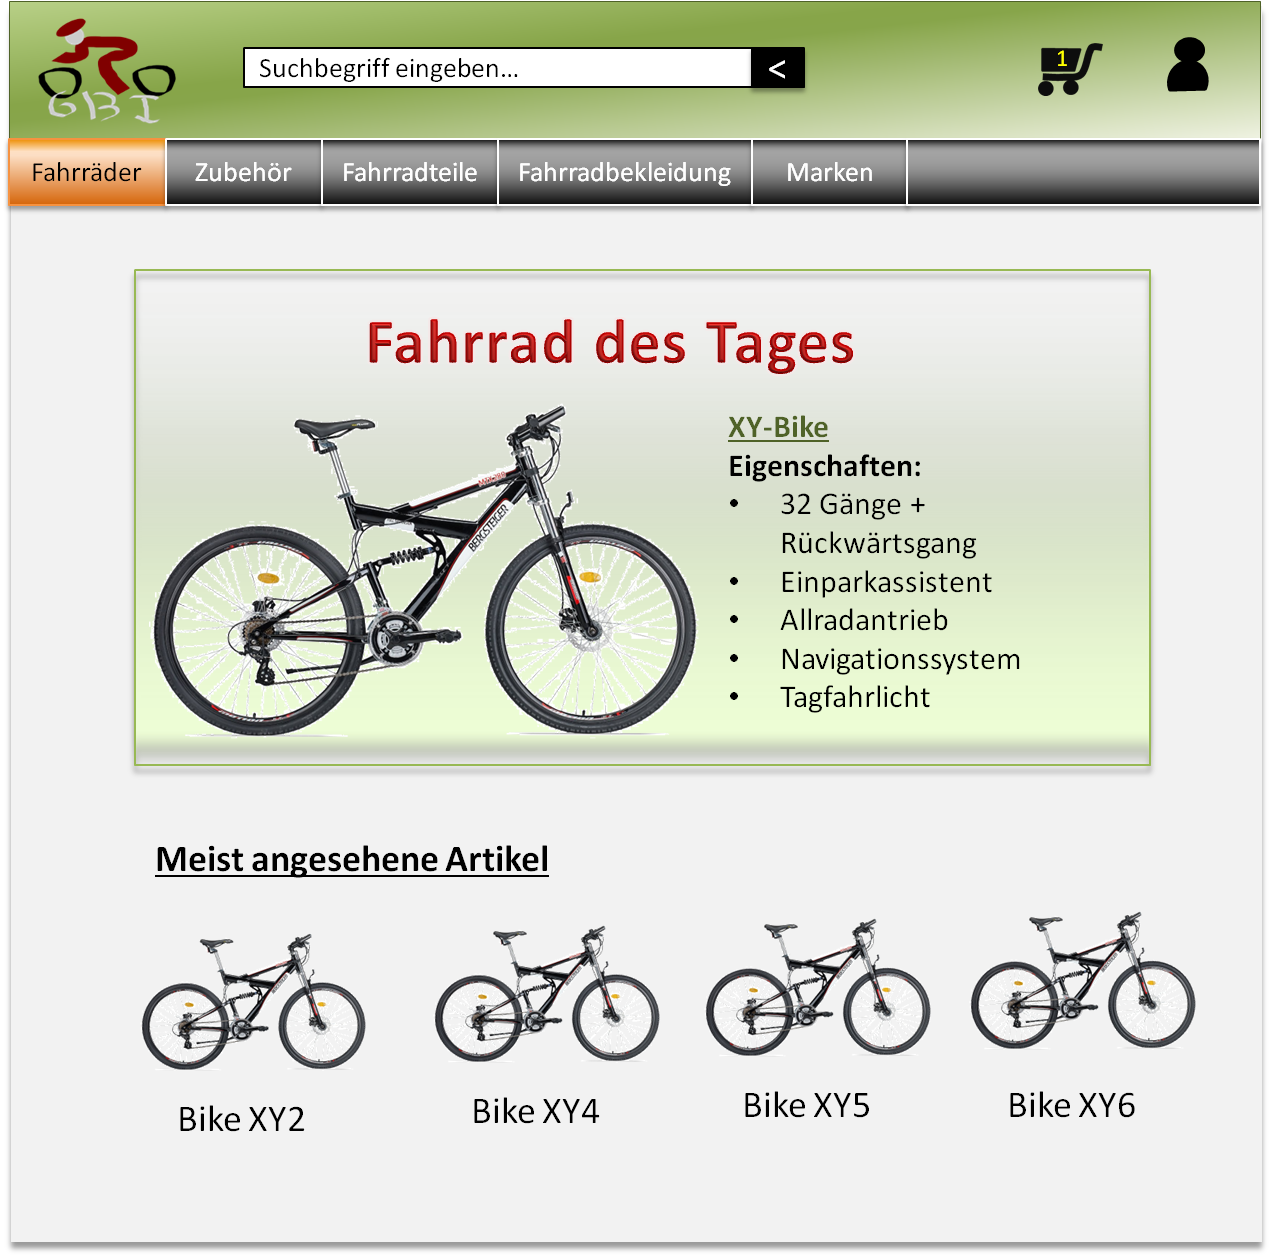
\includegraphics[width=150mm]{Bilder/Abbildung2-GroberDesignEntwurfDesWebshops.png}
\end{center}
\caption{Erster grober Designentwurf der Startseite}
\end{figure}

\subsubsection{Startseite des Webshops}

Die Startseite wird zunächst mit zwei einfachen Artikeln versehen. Sie sollen eine grobe Vorstellung liefern, wie die fertige Startseite aussehen könnte.

\subsubsection{Seitennavigation}

In den darauf folgenden Wochen liegt der Fokus auf die Seitennavigation in der Kopfzeile (nachfolgend Header) der Seite. Die Seitennavigation wird mithilfe von CSS an den Designentwurf angepasst. Es werden die Hauptkategorien „Fahrräder“, „Zubehör“, „Fahrradteile“, „Fahrradbekleidung“, „Marken“ und eine Rubrik „HowTo“ angezeigt. Letztere verlinkt auf eine Internetquelle, mit dessen Hilfe die Seitennavigation umgesetzt wurde. Diese Kategorie dient den anderen Gruppenmitgliedern als Referenz und wird in späteren Versionen des Webshops wieder entfernt. Fährt der Nutzer mit der Maus über die Kategorie „Fahrräder“ öffnet sich ein Drop-Down-Menü, welches den Nutzer verschiedene Fahrradmodelle auswählen lässt. Die komplette Seitennavigation wurde in CSS3 umgesetzt. CSS3 kann von nahezu jeden aktuellen Browser gelesen werden und bietet zudem den Vorteil, dass der entsprechende Code in der bisherigen CSS-Datei eingefügt werden kann. Da CSS3 unabhängig von Java Script ist, lässt sich die Seite zudem problemlos bedienen, wenn Java Script auf den jeweiligen Browsern deaktiviert ist. Dies begründet die Entscheidung CSS3 für die Seitennavigation zu verwenden.
<<<<<<< HEAD
Abbildung 3 und 4 zeigen den bisherigen Seitenprototypen:
=======
\textit{Abbildung 6} und \textit{7} zeigen den bisherigen Seitenprototypen:
>>>>>>> refs/remotes/origin/master



\begin{figure}[H]
\begin{center}
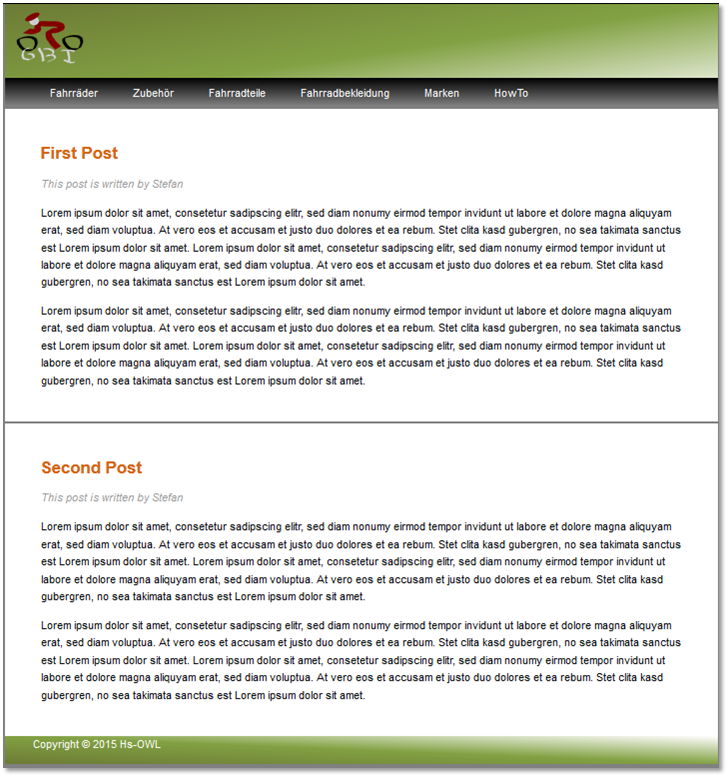
\includegraphics[width=150mm]{Bilder/Abbildung3-Seitenprototyp.png}
\end{center}
\caption{Seitenprototyp}
\end{figure}


\begin{figure}[H]
\begin{center}
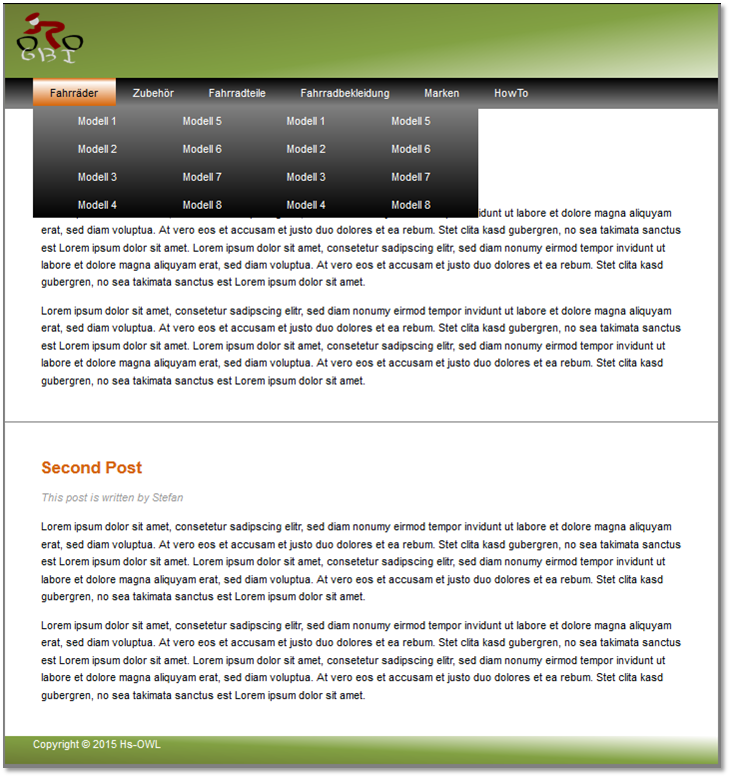
\includegraphics[width=150mm]{Bilder/Abbildung4-SeitenprototypMitDropDownMenue.png}
\end{center}
\caption{Seitenprototyp mit Drop-Down-Menü}
\end{figure}



%Ein paar Wochen später wird sich dazu entschlossen das Programm „Eclipse“ zum Programmieren des Webshops zu nutzen. Das Programm bietet neben einer Autovervollständigung und der Unterstützung mehrerer Programmiersprachen noch zusätzlich den Vorteil, dass es durch Plug-Ins erweiterbar ist. So lässt sich „Eclipse“ durch das Plug-In „GitHub“ erweitern. „GitHub“ ist eine Cloud basierte Lösung zum gemeinsam bearbeiten von Programmcode. Das komplette Projekt wird dabei auf einen Server hochgeladen. Jedes Gruppenmitglied, das einen Acount bei „GitHub“ erstellt hat, kann dem Projekt beitreten, indem es bei den Gruppen- Administrator um Erlaubnis bittet. Dadurch kann ein Dokument von mehreren Gruppenmitgliedern gemeinsam bearbeitet werden. So entstehen mehrere Versionen von einem Dokument, die anschließend wieder zu einem Dokument zusammengefügt werden können.%
<<<<<<< HEAD

\subsubsection{Weitere Arbeiten an der Startseite des Webshops}

Im Laufe der nächsten Woche wird die Startseite des Webshops gemäß dem Designentwurfs erstellt (siehe Abbildung 4). Auf der Startseite ist das „Angebot des Tages“ zu sehen. Es gibt eine Kurzbeschreibung zu dem Artikel mit den wichtigsten Eigenschafen. Der untere Teil der Startseite zeigt die meist angesehenen Artikel des Nutzers an. 
=======
Im Laufe der nächsten Woche wird die Startseite des Webshops gemäß dem Designentwurfs erstellt (siehe \textit{Abbildung 8}). Auf der Startseite ist das „Angebot des Tages“ zu sehen. Es gibt eine Kurzbeschreibung zu dem Artikel mit den wichtigsten Eigenschafen. Der untere Teil der Startseite zeigt die meist angesehenen Artikel des Nutzers an. 
>>>>>>> refs/remotes/origin/master

\begin{figure}[H]
\begin{center}

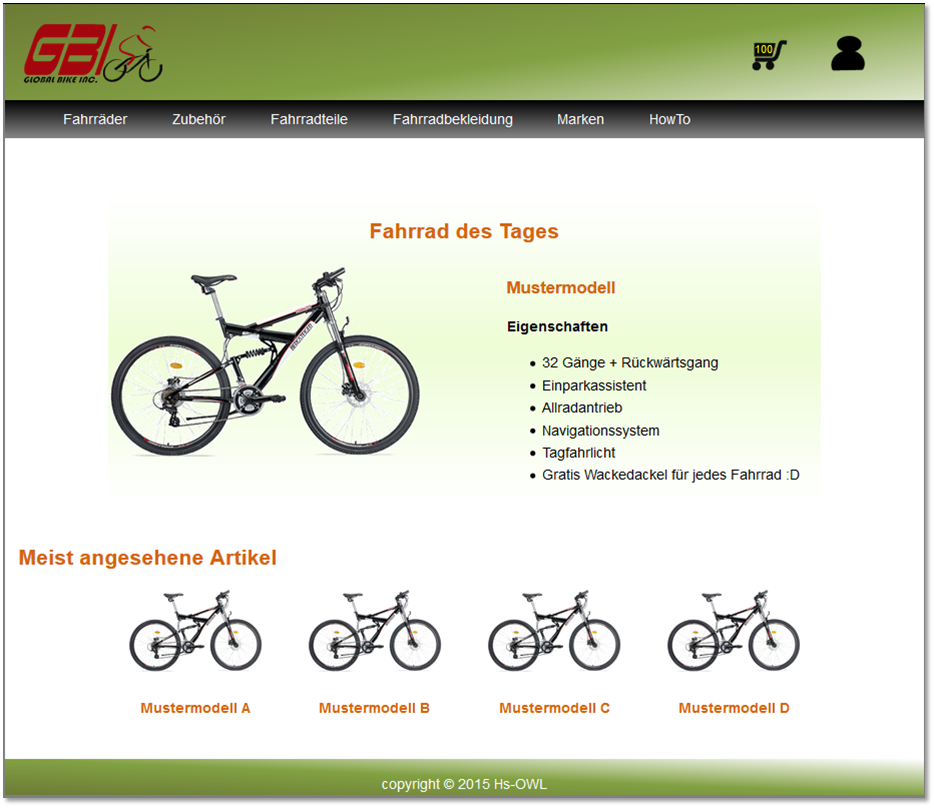
\includegraphics[width=150mm]{Bilder/Abbildung5-StartseiteDesWebshops.png}
\end{center}
\caption{Startseite des Webshops}
\end{figure}


\subsubsection{Rechtsschutz}

In den nächsten Tagen wird das Thema Rechtsschutz behandelt. Dem Webshop werden ein Impressum, die AGB sowie Hinweise zum Datenschutz hinzugefügt:

\begin{figure}[H]
\begin{center}
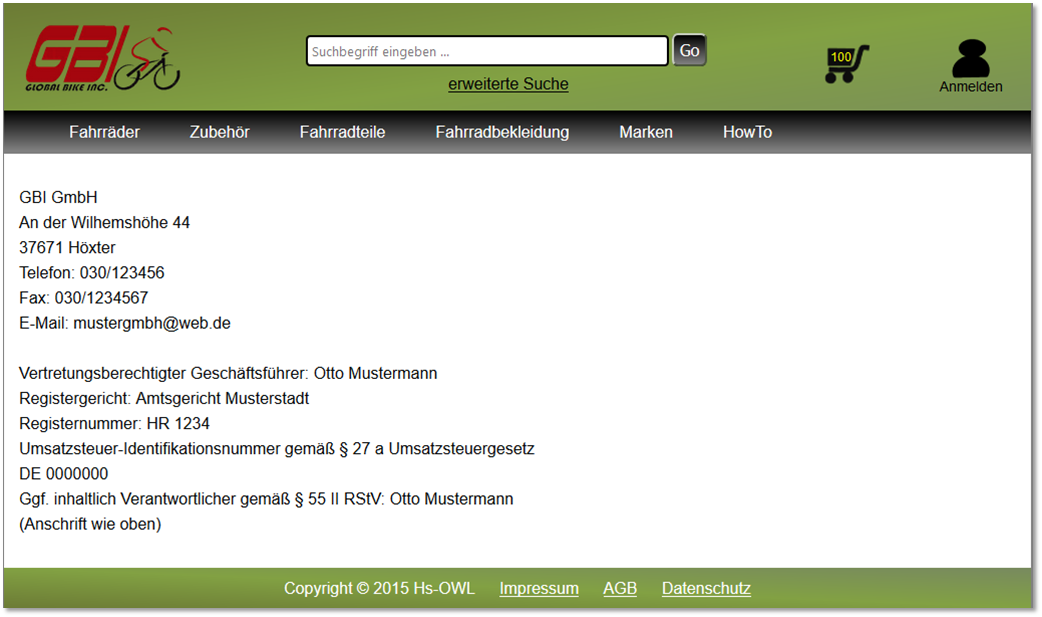
\includegraphics[width=150mm]{Bilder/Abbildung6-ImpressumDesWebshops.png}
\end{center}
\caption{Impressum des Webshops}
\end{figure}

\begin{figure}[H]
\begin{center}
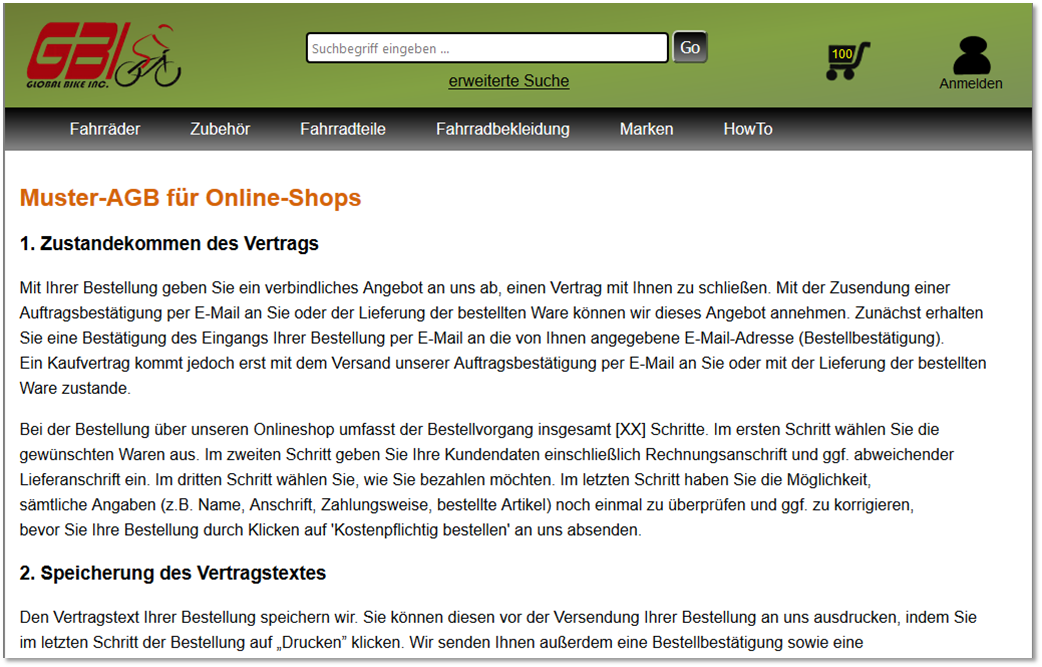
\includegraphics[width=150mm]{Bilder/Abbildung7-AGBDesWebshops.png}
\end{center}
\caption{AGB des Webshops}
\end{figure}

\begin{figure}[H]
\begin{center}
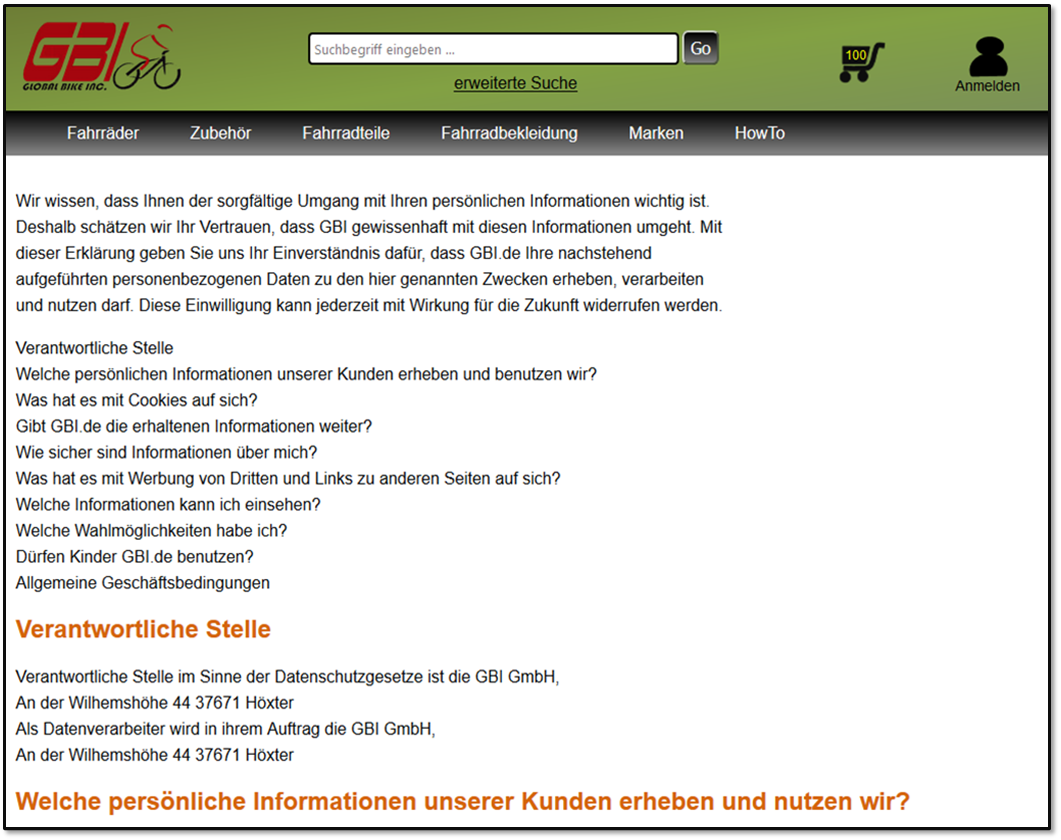
\includegraphics[width=150mm]{Bilder/Abbildung8-DatenschutzDesWebshops.png}
\end{center}
\caption{Datenschutz des Webshops}
\end{figure}

\subsubsection{Dynamische Seitennavigation}

In den nächsten Wochen wird der statische Inhalt des Webshops durch dynamischen Inhalt ersetzt. Das bedeutet, dass die Daten fortan aus einer Datenbank geladen werden. Diese Datenbank wird mit der Datenbank aus dem SAP- System synchronisiert. Zunächst wird die Navigation des Webshops durch dynamische Inhalte ersetzt. Wird nun eine neue Haupt- oder Unterkategorie hinzugefügt oder entfernt, ändert sich die Navigation entsprechend. Zum besseren Verständnis ein kurzes Beispiel: Angenommen die GBI würde jetzt auch Helmkameras anbieten, so würde in der Datenbank eine neue Kategorie „Helmkameras“ erstellt und zur ihr Kameramodelle von „GoPro“ und „Rollei“. Die Navigation hätte jetzt die Hauptkategorien „Fahrräder“, „Zubehör“, „Fahrradteile“, „Fahrradbekleidung“ und die Hauptkategorie „Helmkameras“. Unter letzterer würden die beiden Unterkategorien „GoPro“ und „Rollei“ aufgeführt. Abbildung 8 zeigt die dynamische Navigation:

\begin{figure}[H]
\begin{center}
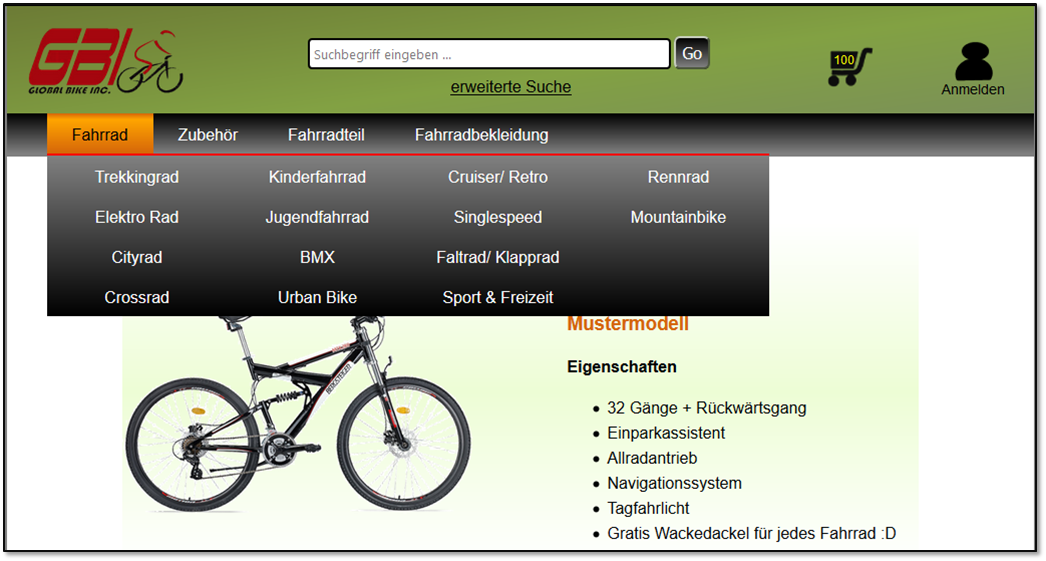
\includegraphics[width=150mm]{Bilder/Abbildung9-DynamischeNaviagtionDesWebshops.png}
\end{center}
\caption{Dynamische Navigation}
\label{Abbildung9-Dynamische Navigation}
\end{figure}


\subsubsection{Dynamische Artikelauflistung}

Ein paar Tage später erstellt Herr Schnürer eine dynamische Artikelauflistung. In ihr werden alle Fahrräder einer bestimmten Kategorie aufgelistet. Wählt der Nutzer in der Seitennavigation die Hauptkategorie „Fahrrad“ und anschließend die Unterkategorie „Cityrad“ werden ihm alle „Cityräder“ aufgelistet, wählt er die Unterkategorie „Mountainbike“ werden ihm alle „Mountainbikes“ aufgelistet usw. Abbildung 9 zeigt die dynamische Artikelauflistung aller „Cityräder“ (Anmerkung: Es wird an dieser Stelle nur ein Cityrad aufgelistet, da sich nur ein Produkt mit der Kategorie „Cityrad“ in der Datenbank befindet. Man müsste nur weitere Cityräder in der Datenbank hinterlegen, damit entsprechend mehr Produkte aufgelistet werden):

\begin{figure}[H]
\begin{center}
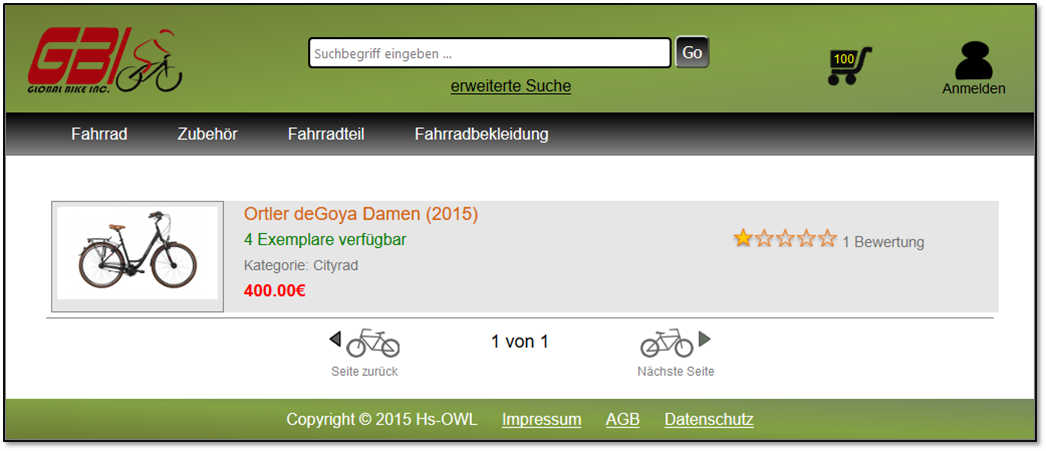
\includegraphics[width=150mm]{Bilder/Abbildung10-DynamischeArtikelauflistungAllerCitybikes.png}
\end{center}
\caption{Dynamische Artikelauflistung aller Cityräder}
\label{Abbildung10-Dynamische Artikelauflistung aller Cityräder}
\end{figure}


\subsubsection{Detaillierte dynamische Artikelbeschreibung}

Eine Woche später wird eine detaillierte und dynamische Beschreibung für die Artikel erstellt. Wählt der Nutzer einen Artikel aus, erscheint eine detaillierte Beschreibung dessen. Der oberer Teil ist dabei an die Artikelbeschreibung der Startseite angelehnt und zunähst noch statisch, der untere Teil beschreibt den Artikel näher und ist bereits dynamisch umgesetzt. So erscheint unter der Überschrift „Artikelbeschreibung“ die jeweilige Beschreibung des zuvor ausgewählten Artikels. Abbildung 10 zeigt eine solche Beschreibung für das Fahrrad „Ortler deGoya Damen (2015)“:

\begin{figure}[H]
\begin{center}
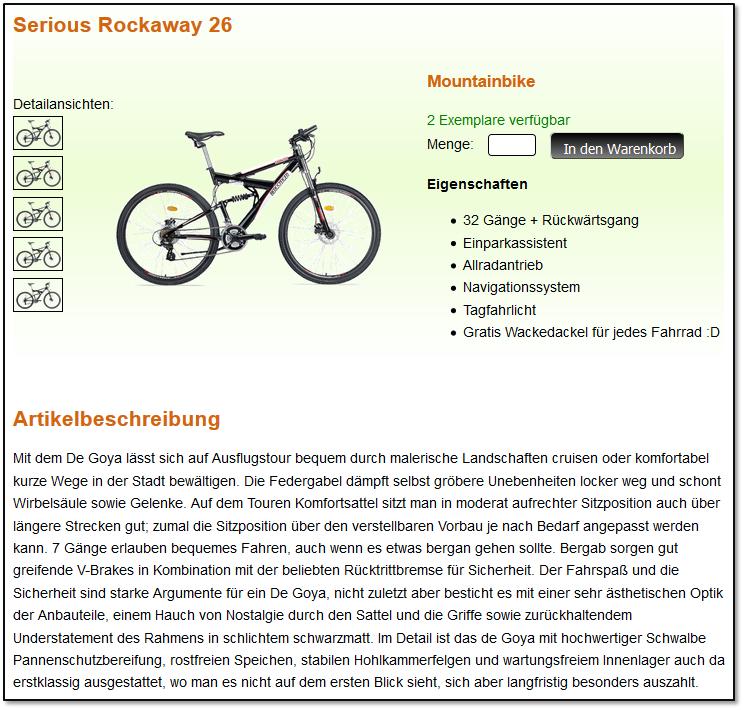
\includegraphics[width=150mm]{Bilder/Abbildung11-DynamischeDetailierteArtikelbeschreibung.png}
\end{center}
\caption{Detaillierte dynamische Artikelbeschreibung}
\label{Abbildung11-Detaillierte dynamische Artikelbeschreibung}
\end{figure}

Wie bereits erwähnt ist der obere Teil zunähst nur statisch programmiert worden, weshalb die Überschrift noch nicht zum ausgewählten Artikel passt. Der Text „Artikelbeschreibung“ hingegen wird bereits aus der Datenbank geladen.
\\
In den Sommersemesterferien hat Herr Schnürer auch den oberen Teil dieser Seite dynamisch erstellt. Die Produktbilder und Eigenschaften des Artikels werden nun ebenfalls aus der Datenbank geladen. Zudem wird noch ein kleines Extra eingebaut: Klickt der Nutzer eines der Produktbilder an, wird mithilfe eines Java Scripts eine „lightbox“ aufgerufen. Diese zeigt die Produktbilder in ihrer normalen Auflösung und ermöglicht das einfache Durchklicken der Produktbilder. Abbildung 12 zeigt den fertigen oberen der der Artikelbeschreibung, während Abbildung 13 die „lightbox“ veranschaulicht:

\begin{figure}[H]
\begin{center}
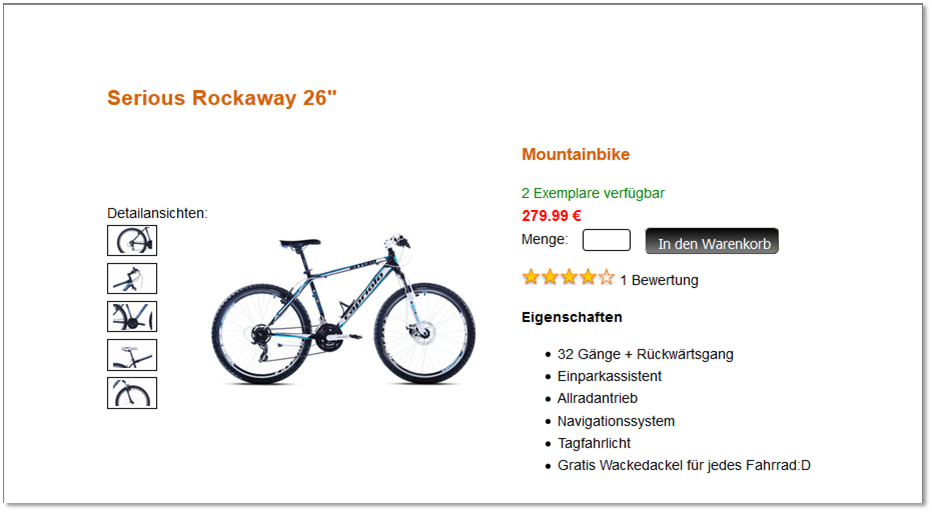
\includegraphics[width=150mm]{Bilder/Abbildung12-DynamischeDetailierteArtikelbeschreibungFertig.png}
\end{center}
\caption{Abbildung 12 Fertige dynamische Artikelbeschreibung}
\label{Abbildung12-Fertige dynamische Artikelbeschreibung}
\end{figure}

\begin{figure}[H]
\begin{center}
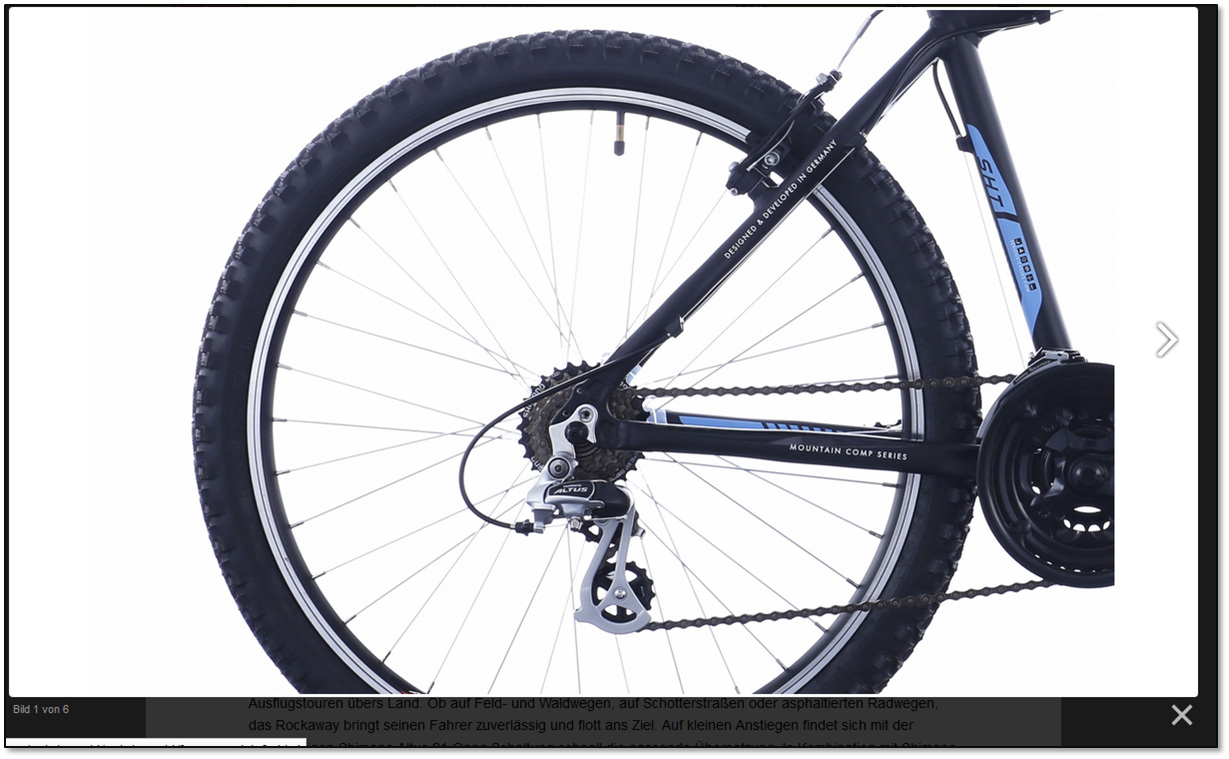
\includegraphics[width=150mm]{Bilder/Abbildung13-Lightbox.png}
\end{center}
\caption{Abbildung 13 "Lightbox" zur besseren Darstellung der Produktbilder}
\label{Abbildung13-"Lightbox" zur besseren Darstellung der Produktbilder}
\end{figure}





\subsection{Arbeitspakete von Herrn Brüntrup}
In diesen Abschnitt wird beschrieben, wie Herr Brüntrup seine Arbeitspakete gelöst hat. Zudem wird in diesen Abschnitt noch beschrieben welche Arbeitspakete wegen Zeitmangel und fehlender Arbeitsbereitschaft zusätzlich noch übernommen wurden.

\subsubsection{Arbeitspaket 5: Die Schnittstellendatenbank}
Die Datenbank stellt die Schnittstelle zwischen den SAP-System und den Webshop da. Aus diesem Grund wurde die Datenbankstruktur in der ersten Woche nach der Arbeitspaketverteilung zusammen mit Mitgliedern der SAP-Gruppe entworfen.\\

\textbf{Gründe für die Schnittstellendatenbank}\\
Die Gründe warum die Kommunikation mit einer Schnittstellendatenbank gelöst wurde wird in den folgenden Sätzen genannt. Der erste Grund war die Verfügbarkeit. Der Webshop sollte auch erreichbar sein, wenn mal keine Verbindung zum SAP-System besteht. Der SAP-Server steht extern bei einer Hochschule in Magdeburg. Es könnte also schon mal dazu kommen, dass das System nicht erreichbar ist. Ein anderer Grund war die Flexibilität. Die Datenhaltung sollte flexible erweiterbar sein. Soll die Webseite erweitert werden, z.B. durch eine 360$^\circ$-Ansicht des Fahrrads,kann einfach die benötigten Felder zur Datenbank hinzugefügt werden. Beim SAP-System ist das nur beschränkt möglich. Der Zugriff auf das SAP-System wird mit vordefinierten Funktionen gelöst. Dieses Funktionen werden \glqq Business Application Programming Interface (BAPI)\grqq{} genannt. Da die SAP-Gruppe beim SAP-System keine Berechtigungen hat neue BAPIs zu erstellen wäre somit die Erweiterbarkeit des Webshops sehr eingeschränkt.\\

\textbf{Aufbau der Schnittstellendatenbank}\\
Nun wird der zu Beginn geplante Aufbau der Schnittstellendatenbank erläutert. Die zu Beginn geplante Datenbank bestand aus den Relationen \glqq Kunde\grqq{}, \glqq Bestellungen\grqq{}, \glqq Produkte\grqq{} und \glqq Produktbilder\grqq{}. Die Relation \glqq Kunde\grqq{} enthält die Login-Daten des Kunden, sowie dessen Adresse. Die Relation \glqq Bestellungen\grqq{} enthält alle Angaben zur Bestellung. Angaben sind z.B. die Zahlungs- und Versandart, sowie der Status der Bestellung. Die vorletzte genannte Relation beinhaltet alle Angaben zu den Produkten, die beim Webshop verkauft werden sollen. Ihr wurde deswegen auch den Namen \glqq Produkte\grqq{} gegeben. Die Relation \glqq Produktbilder\grqq{} enthält Pfadangaben, wo auf den Server die Produktbilder abgelegt sind. Da zu einen Produkt mehrere Produktbilder abgelegt werden können wurde sich auf eine extra Tabelle für die Produktbilder geeinigt.

Eine Relation, die die Produkte einer Bestellung enthält wurde zunächst vergessen umzusetzen. Das Vergessen der Relation fiel erst auf, als die SAP-Gruppe mit der Umsetzung des Bestellvorgangs bei der SAP-Schnittstelle beginnen wollte. Zur Lösung des Problems fügte die SAP-Gruppe nun nachträglich eine Relation \glqq Bestellprodukte\grqq{} zur Datenbank hinzu. Dieses Relation steht in Beziehung mit den Relationen \glqq Bestellungen\grqq{} und \glqq Produkte\grqq{}. Die Relation beinhaltet die Produkte einer Bestellung.

Als Datenbank-Server wurde sich auf MYSQL geeinigt. Dieser Server lässt sich problemlos auf Linux installieren. Es war wichtig, dass die Datenbank unter Linux läuft, da die Server-Gruppe einen Linux-Server aufsetzen wollte. Zudem bietet MYSQL den Vorteil, dass auf eine MYSQL-Datenbank mit der Programmiersprache PHP gut zugegriffen werden kann. Die SAP-Gruppe wollte die Datenbank mit einer selbst geschriebenen JAVA-Anwendung füllen. Auch von JAVA aus kann gut auf eine MYSQL-Datenbank zugegriffen werden. Ein weiterer Grund für die Nutzung der MYSQL-Datenbank war, dass die Softwaresammlung XAMPP einen MYSQL-Server beinhaltet. Die Softwaresammlung XAMPP wurde von der Webshop-Gruppe als Testserver zum Testen der Webseite auf den Hochschulrechnern verwendet. \\
Die \textit{Abbildung 12} zeigt das \glqq Entity-Relationship-Diagramm (ERD)\grqq{}. Dieses Diagramm ist die erste Version der Datenbank, die zusammen mit der SAP-Gruppe entworfen wurde. 

\begin{figure}[H]
	\begin{center}
		\fbox{
			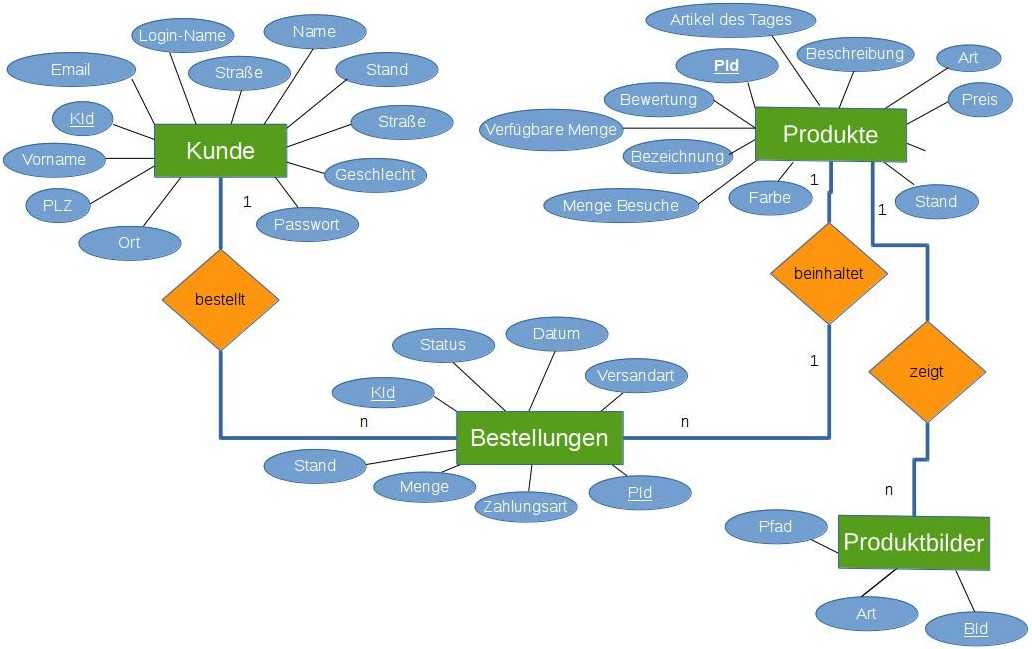
\includegraphics[width=150mm]{Bilder/Abbildung10-erd_alt.jpg}
		}
	\end{center}
	\caption{Erster Datenbankentwurf}
\end{figure}

Da es ursprünglich bemängelt wurde, dass das Projekt noch nicht den für das Modul benötigten Zeitaufwand aufweisen wurde, wurde beschlossen das Arbeitspaket \glqq Bewertung\grqq{} mit einer Kommentarfunktion zu erweitern. Somit sollte der Kunde auch ein Kommentar für seine Bewertung äußern können. Dafür musste die Datenbank etwas angepasste werden. Vorher war einfach ein Attribut \glqq Bewertung\grqq{} in der Relation \glqq Produkte\grqq{} vorzufinden. Um die Kommentare für die Bewertung speichern zu können wurde die Datenbank um eine Relation \glqq Kommentare\grqq{} erweitert. Dieses Relation beinhaltet ein Datenfeld, wo die Bewertung des Kunden (von 1-5 Sterne) und eins wo Bewertungstext gespeichert wird. \\
Als mit der Suchfunktion und der Navigation begonnen wurde fiel schnell auf, dass benötigte Attribute und Tabellen für die Navigation vergessen wurden. Somit wurde eine neue Relation \glqq Produktkategorie\grqq{} zur Datenbank hinzugefügt. Dieses Relation steht mit der Relation \glqq Produkte\grqq{} in Beziehung und beinhaltet alle Produktkategorien, die der Webshop anbieten soll. Unter Produktkategorien wird beim Webshop die Festlegung verstanden, ob das Produkt ein Ersatzteil, ein Fahrrad, Zubehör usw. ist. Eine zweite Relation, die mit der Relation Produkte in Beziehung steht, ist die Relation \glqq Bauart\grqq{}. Dieses Relation wird nur verwendet, wenn das Produkt ein Fahrrad ist. In dieser Relation sind alle beim Webshop angebotenen Bauarten aufgelistet. Unter Bauart wird bei diesen Webshop verstanden, ob es sich um ein Mountenbike, Trekkingbike usw. handelt.

Die \textit{Abbildung 13} zeigt die endgültige Struktur der Schnittstellendatenbank mit allen nachträglich hinzugefügten Relationen. 
\begin{figure}[H]
	\begin{center}
		\fbox{
			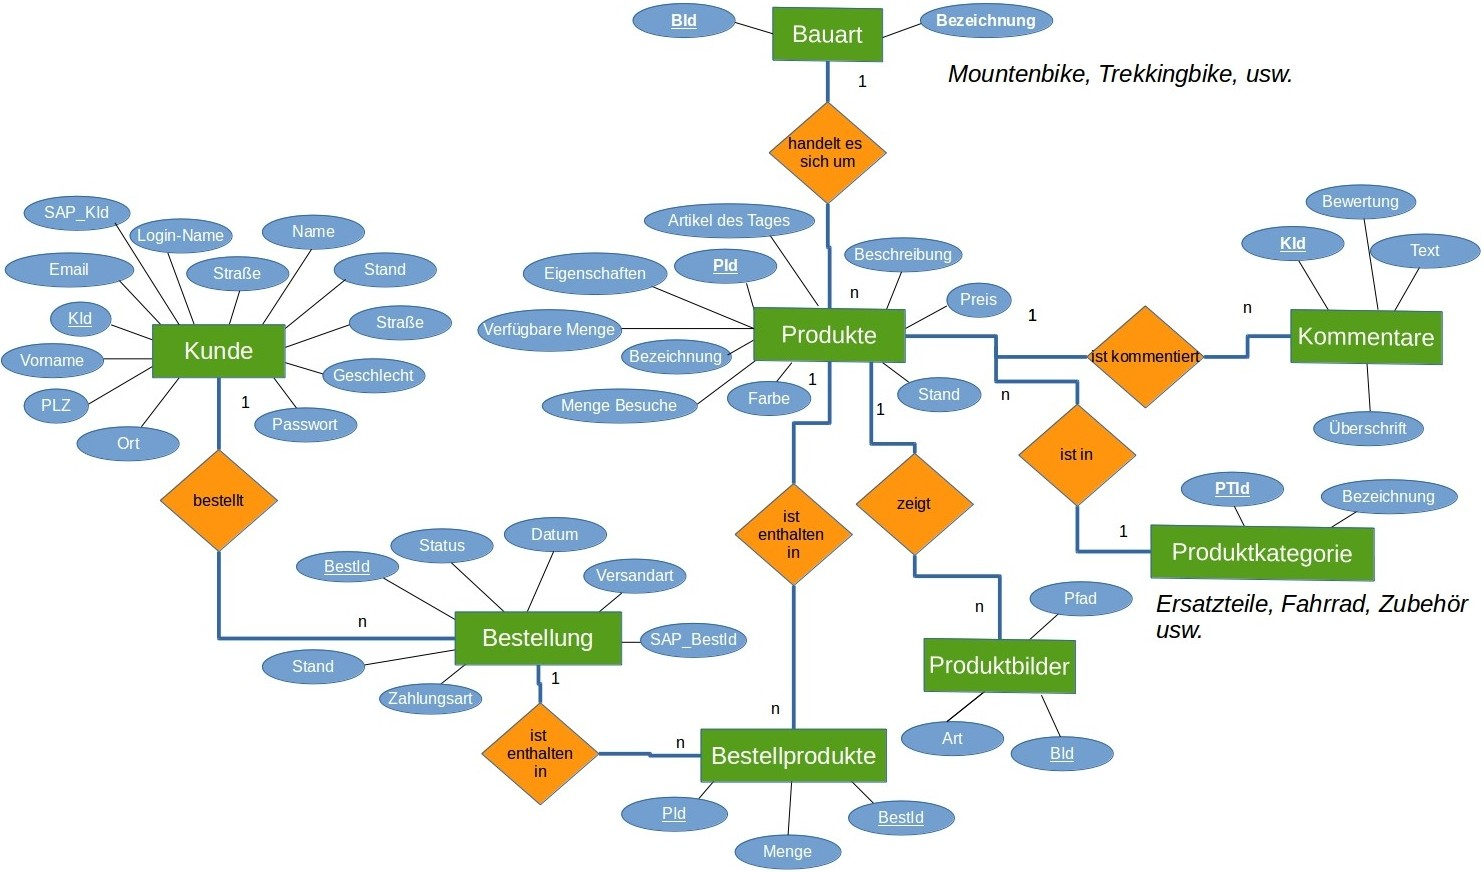
\includegraphics[width=150mm]{Bilder/Abbildung11-erd.jpg}
		}
	\end{center}
	\caption{Endgültiger Datenbankentwurf}
\end{figure}

\textbf{Wahl der PHP-API zum Datenbankzugriff}\\
Um von PHP aus auf eine MYSQL-Datenbank zugreifen zu können gibt es mehrere Möglichkeiten. In dieser Ausarbeitung werden die Zugriffsmöglichkeiten kurz verglichen und dann erläutert welche davon für das Projekt benutzt wurde.

Die erste Möglichkeit ist die PHP-API \glqq ext/mysql \grqq{}. Diese API ist veraltet und wird nicht mehr weiterentwickelt. Sie unterstützt noch nicht alle MYSQL 5.1+ Funktionalitäten und ist stellenweise mit neuen PHP-Versionen nicht mehr nutzbar. Dieses Erweiterung nutzt den prozeduralen Ansatz. Die nächste Möglichkeit ist die PHP-API \glqq PDO\grqq{}. Diese API unterstützt fast alle Funktionalitäten von MYSQL 5.1+. Sie bietet zudem den Vorteil, dass die API auch zum Zugriff auf andere SQL-basierten Datenbanken genutzt werden kann. Diese API hat einen objektorientierten Aufbau.  Die letzte Zugriffsmöglichkeit bietet die API \glqq ext/mysqli\grqq{}. Sie unterstützt alle MYSQL 5.1+ Funktionalitäten und kann objektorientiert und prozedural programmiert werden.

Die Auswahl fiel auf die API \glqq ext/mysqli\grqq{}. Die Gründe hierfür waren, dass die API alle Funktionalitäten der neusten MYSQL-Version unterstützt, regelmäßig auf die neuesten MYSQL-Funktionen angepasst wird und schon Quellcode von alten Projekten übernommen werden konnte. Die \textit{Abbildung 14} zeigt die Eigenschaften der drei APIs nochmal in einer Tabelle zusammen gefasst.
\begin{figure}[H]
	\begin{center}
		\fbox{
			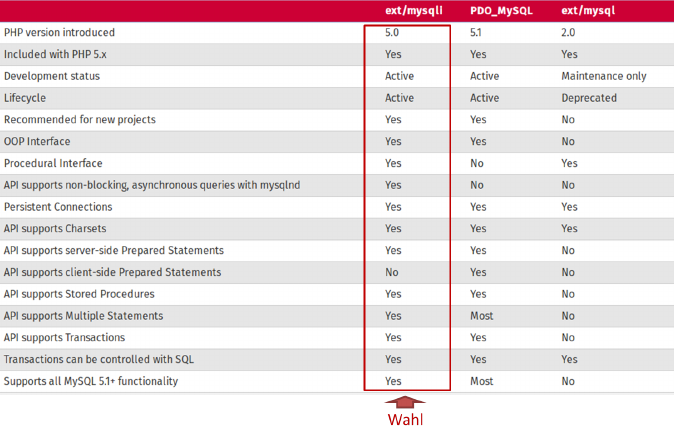
\includegraphics[width=150mm]{Bilder/Abbildung12-mysql_apis.png}
		}
	\end{center}
	\caption{Überblick der PHP-APIs zum Datenbankzugriff}
\end{figure}

\textbf{Die Konfigurationsdatei}\\
Um auf eine MYSQL-Datenbank zugreifen zu können werden üblicherweise mehrere Zugangsdaten benötigt. Die Zugangsdaten, die mindestens benötigt werden sind der Datenbankbenutzername, das Passwort zum Benutzername, der Datenbankname und die IP-Adresse des Servers. Damit diese Zugangsdaten nicht bei jeden Datenbankzugriff im Quelltext angegeben werden müssen, wurden diese Angaben in eine Konfigurationsdatei ausgelagert. Wird die Webseiten später mal auf einen anderen Webserver betrieben, so müssen die Datenbankzugangsdaten nur in dieser Datei geändert werden. Die Konfigurationsdatei ist extra gesichert worden, damit sie nicht direkt im Browser geöffnet werden kann. Der Datei wurde als Dateiendung \glqq *.php.inc\grqq{} angehangen. Mit einer bestimmten Zeile in einer Konfigurationsdatei für den Webserver wurde das Öffnen von \glqq *.inc\grqq{}-Dateien den Browser untersagt. Die Konfigurationsdatei trägt den Namen \glqq .htaccess\grqq{} und befindet sich im Home-Vezeichnis der Webseite. Mehr zur \glqq .htaccess\grqq{}-Datei kann im Abschnitt \glqq Webshopsicherheit\grqq{} gelesen werden.

Der \textit{Quellcode 1} zeigt die Konfigurationsdatei des Webshops. In dieser Datei sind die benötigten Datenbankzugangsdaten und die festgelegte Email-Adresse zu lesen, von der alle Bestätigungs-Emails versendet werden sollen. Zudem sind in der Konfigurationsdatei die Bankdaten definiert, die den Kunden mitgeteilt werden, wenn er als Zahlungsart \glqq Vorkasse\grqq{} ausgewählt hat.

\newpage
\begin{center}
	\begin{lstinputlisting}[language=PHP, caption={Die Konfigurationsdatei}]
		{Quellcode/config.php.inc}
	\end{lstinputlisting}
\end{center}

\textbf{Die Datenbankzugriffsklasse}\\
Beim Webshop wird nicht direkt über die \glqq MYSQLi\grqq{}-API auf die MYSQL-Datenbank zugegriffen. Es wurde für den Datenbankzugriff extra eine Klasse entwickelt, die als Schnittstelle zwischen den Webshop und der \glqq MYSQLi\grqq{}-API fundiert. Diese Klasse bestand schon von alten Projekten und wurde aus folgenden Grund entwickelt. Sie entstand zu den Zeitpunkt, als die PHP-Entwickler auf der PHP eigenen Webseite bekanntgaben, dass das Standard-MYSQL-API nicht mehr mit den nächsten PHP-Versionen unterstützt werden soll. Somit wurde entschlossen eine Klasse zu entwickeln, dass bei ähnlicher Situation der Nachfolger-API einfach nur der Quelltext in der Klasse geändert werden muss und nicht im ganzen Projekt überall bei gleicher Situation die API ersetzt werden muss. Zudem bietet die Klasse auch einen Vorteil, wenn zu einen späteren Zeitpunkt mal ein anderes Datenbanksystem verwendet werden soll. Bei dieser Situation müsste wie beim vorherigen Beispiel auch nur die Klasse verändert werden und nicht das ganze Projekt.

\newpage
\subsubsection{Arbeitspaket 6: Registrierungs- und Anmeldungsfenster designen und programmieren}
Dieser Abschnitt beschreibt, wie beim Webshop die Registrierung und Anmeldung umgesetzt wurde. Zudem wird die Umsetzung einer Funktion des Webshops beschrieben, wo der Kunde seine Profildaten ändern kann.\\

\textbf{Der Registrierungsvorgang}\\
Auf dieser Webseite läuft die Registrierung, wie in den folgenden Sätzen beschrieben ab. Zunächst tippt der Neukunde die von der Webseite verlangten persönlichen Informationen in ein Formular ein und bestätigt die Eingabe durch einen Klick auf den Bestätigungsbutton. Wenn beim Webbrowser des Neukunden JavaScript nicht deaktiviert ist, überprüft der Webbrowser mit einen JavaScript die Eingabe bevor sie zum Webserver weitergeleitet wird. Die Eingabe wird nur weitergeleitet, wenn dieses vom JavaScript aus als gültig anerkannt wurde. Bei ungültiger Eingabe wird auf der Webseite eine Fehlermeldung ausgegeben. Der JavaScript ist keine endgültige Eingabeüberprüfung, dieser dient nur dafür unnötigen Datenverkehr zu minimieren. JavaScript besitzt den Nachteil, dass dieser beim Webbrowser deaktiviert werden kann. Bei deaktivierten JavaScript wird somit die Eingabe unüberprüft an den Webserver weitergeleitet. Somit muss die Eingabe nochmal beim Webserver auf Gültigkeit überprüft werden.  Der Neukunde wird also erst in die Kunden-Tabelle der Datenbank geschrieben, wenn die serverseitig programmierten Überprüffunktionen die Eingabe als gültig angesehen haben. Wurde die Eingabe als ungültig anerkannt, so wird auch bei der serverseitigen Programmierung eine Fehlermeldung auf der Webseite angezeigt. Nachdem der Kunde erfolgreich in der Kundendatenbank angelegt wurde, bekommt der Neukunde eine Bestätigungsmail zu gesendet. Der Neukunde kann sich erst erfolgreich am System anmelden, wenn dieser den in der Email enthaltenden Link ausgeführt hat. 

Das Passwort des Kunden wird nicht in Klartext in die Datenbank gespeichert. Bevor es in die Datenbank geschrieben wird, wird das Passwort mit einen \glqq MD5-Hash-Algorithmus\grqq{} unkenntlich gemacht. Der MD5-Hashwert ist nicht mit einen Schlüssel wieder invertierbar. Er kann zur Speicherung von Passwörtern verwendet werden, da beim \glqq MD5-Hash-Algorithmus\grqq{} der gleiche Input immer den gleichen Output erzeugen. Somit wird beim Login-Check einfach auch das eingegebene Passwort unkenntlich gemacht und verglichen, ob es mit den Wert in der Datenbank übereinstimmt.\\ Die \textit{Abbildung 15} zeigt den Registrierungsvorgang nochmal als BPMN dargestellt.\\

\begin{figure}[H]
	\begin{center}
			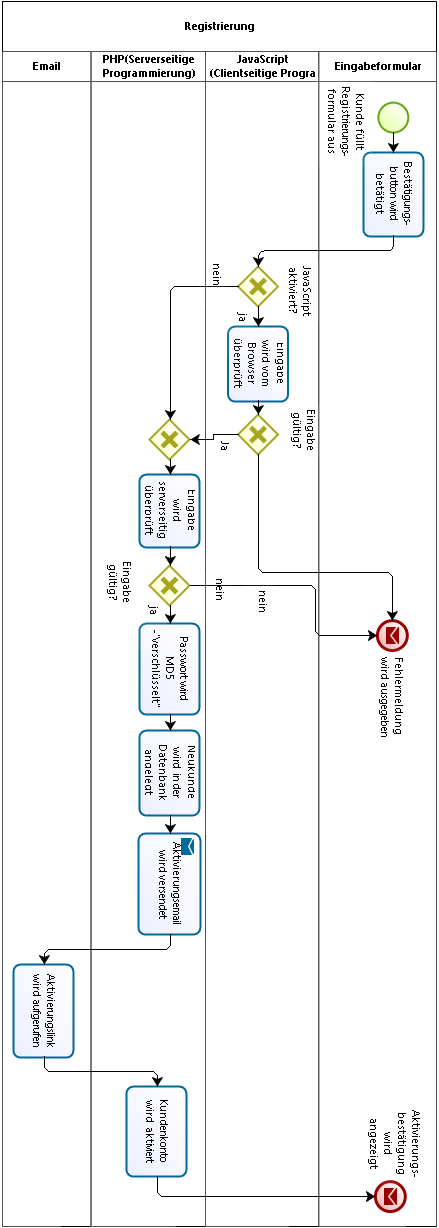
\includegraphics[width=225pt]{Bilder/Abbildung13_Reg_Vorgang.png}
	\end{center}
	\caption{Der Registrierungsvorgang}
	\label{fig:Abbildung 13}
\end{figure}


\textbf{Der Anmeldungsvorgang}\\
Der Anmeldungsvorgang läuft ähnlich wie der Registrierungsvorgang ab. Der Kunde tippt als Benutzernamen seine Email-Adresse und als Passwort das bei der Registrierung angegebene Passwort in das Anmeldeformular ein. Wie bei der Registrierung überprüft ein JavaScript die Eingabe, bevor diese an den Server weitergeleitet wird. Die vorherige Überprüfung ist wieder nur bei aktivierten JavaScript im Webbrowser möglich. Deswegen wird die Überprüfung bei der Anmeldung auch nochmal vom Server überprüft. Hat der Kunde eine gültige Eingabe getätigt, so wird die Email-Adresse und das Passwort mit den Datensätzen in der Kunden-Tabelle der Datenbank verglichen. Um den Vergleich ausführen zu können wird bei der Anmeldung auch das Passwort durch den  \glqq MD5-Hash-Algorithmus\grqq{} unkenntlich gemacht. Wurde in der Tabelle ein Datensatz gefunden, wo Email-Adresse und Passwort übereinstimmen, so wird der Kunde eingeloggt. Wurde keine Übereinstimmung gefunden, so wird auf der Webseite eine Fehlermeldung ausgegeben.\\ 
Der Einlogvorgang läuft wurde wie folgt umgesetzt. Die Anmelde-Email-Adresse wird in einer SESSION-Variable gespeichert. Der SESSION-Variable wurde den Namen \glqq \$\_SESSION['angemeldet']\grqq{} gegeben. An Hand dieser Variable erkennt der Webshop, ob der Kunde angemeldet ist oder nicht. Wurde die Variable angelegt und enthält einen Wert, so wird dieses als angemeldet interpretiert. Die Abmeldung erfolgt einfach durch das Löschen dieser Variable. Eine SESSION-Variable behält die enthaltenden Daten über mehrere Seitenaufrufe. Wenn nicht mehr auf die Variable zugegriffen wird, werden die Daten dieser Variable automatisch nach einer bestimmten Zeit gelöscht. Ob der Kunde angemeldet ist muss in einer SESSION-Variable zwischengespeichert werden, da das HTTP-Protokoll verbindungslos ist. Es wird also jede HTTP-Anfrage isoliert betrachtet. Ohne die SESSION-Variable könnte sich somit der Webserver nicht merken, dass der Kunde angemeldet ist. Einer Session wird in PHP eine eindeutige \glqq SESSION-ID\grqq{} zugeordnet. Diese SESSION-ID wird entweder als Cookie im Browser abgespeichert oder immer der Seiten-URL mit übergeben. Wird die SESSION-ID in einen Cookie im Browser abgespeichert, so wird diese beim Schließen des Browsers gelöscht. Die Daten, die in der SESSION-Variable abgespeichert sind werden auf der Serverseite zwischengespeichert und nicht im Browser. Die SESSION-ID wird von Browser bei jeder Anfrage an den Server weitergeleitet. An Hand dieser SESSION-ID kann der Server die SESSION-Variable zu den entsprechenden Browser zuordnen.\\

\textbf{Die clientseitige Überprüfung}\\
Wenn JavaScript aktiviert ist, werden, wie oben schon erwähnt, die Formulareingaben zuvor im Browser überprüft. Dafür wird beim Formular den Attribut \glqq onsubmit\grqq{} eine JavaScript-Funktion übergeben. Die Formulareingabe wird hierbei nur an den Server weitergeleitet, wenn diese Methode als Rückgabewert \glqq true\grqq{} zurückgibt. Die JavaScript-Funktion überprüft bei der Eingabe, ob überhaupt ein Text in die Textfelder eingegeben wurde und die Eingabe gültig ist. Zum Beispiel darf eine Postleitzahl nur aus 5 Ziffern bestehen. Die clientseitige Programmierung findet bei der Anmeldung in der Datei \glqq /Funktions/JS/anmeldung.js\grqq{} und bei der Registierung in der Datei \glqq /Funktions/JS/registrierung.js\grqq{} statt.

Der \textit{Quellcode 2} zeigt in vereinfachter Version das Login-Formular. Beim \glqq form\grqq{}-Tag kann das \glqq onsubmit\grqq{}-Attribut gefunden werden. Dieses Attribut startet beim Klick auf den Submit-Button die enthaltende JavaScript-Funktion. Das Attribut lässt nur die Durchführung des Submits zu, wenn die JavaScript-Funktion als Rückgabewert den Wert \glqq true\grqq{} zurückliefert.

Um unnötigen Quelltext zu umgehen, wurde ein Teil des Eingabeüberprüfungsquellcode in eine andere JavaScript-Datei ausgelagert. Der ausgelagerte Quellcode wird bei jeden Formular benötigt. Dieser Quellcode überprüft, ob alle Pflichtfelder ausgefüllt sind. Die ausgelagerte Funktion trägt den Namen \glqq sindAlleFelderAusgefuellt\grqq{} und befindet sich in der Datei \glqq /Funktions/JS/vorcheck\_std\_funktionen.js\grqq{}. Der Funktion wird beim Aufruf drei Parameter übergeben. Der erste Parameter erhält ein Array. Dieses Array enthält die Feldnamen der Textfelder, wovon die Eingabe überprüft werden soll. Der zweite Parameter enthält wiederum ein Array. Dieses Array enthält die Meldungswörter, die in der Fehlermeldung für das jeweilige Textfeld eingesetzt werden sollen. Die Meldungswörter werden in die Fehlermeldung eingesetzt, wenn das Textfeld nicht gefüllt ist. Beim letzten Parameter wird der Name des Formulars angeben, worauf sich die Textfelder befinden. Sind nicht alle Felder ausgefüllt, erstellt die Funktion eine Fehlermeldung und gibt diese als Rückgabewert aus.\\
In die Auslagerungsdatei wurden zudem Funktionen zur Überprüfung der Email-Adresse oder ob die Eingabe eine Zahl ist abgelegt. Die Funktionen in den Dateien \glqq /Funktions/JS/anmeldung.js\grqq{} und  
\glqq /Funktions/JS/registrierung.js\grqq{} rufen die ausgegliederten Funktionen auf und führen noch eine genauere Überprüfung durch. Die Funktionen testen zum Beispiel, ob das Passwort mit der Passwortwiederholung übereinstimmt.
\newpage
\begin{center}
	\begin{lstinputlisting}[language=HTML, caption={Login-Formular (vereinfacht)}]
		{Quellcode/login-formular.php.inc}
	\end{lstinputlisting}
\end{center}

\textbf{Serverseitige Programmierung}\\
Wie bei der clientseitigen Programmierung wurde auch bei der serverseitigen Programmierung die Methode zur Überprüfung, ob alle Pflichtfelder ausgefüllt sind ausgelagert. Bei der serverseitigen Programmierung wurde hierfür die Technik der Vererbung genutzt. Serverseitig wurde der Webshop objektorientiert programmiert. Für die zuvor genannte Methode wurde die Klasse \glqq EingabeCheckGrundlegend\grqq{} erstellt. Dieses Klasse wurde an alle anderen Klassen vererbt, die Formulareingaben entgegen nehmen müssen. Für die Registrierung, Anmeldung und Änderung des Kundenprofils ist die Klasse \glqq Kunde\grqq{} entwickelt worden. Sie enthält Methoden, mit der die Formulareingabe geprüft, ein neuer Kunde angelegt, ein Kunde verwaltet und die Anmeldung durchgeführt werden kann.\\
Instanziiert wird die Klasse durch Skripte des Ordners \glqq /Funktions/PHP\grqq{}. Registriert sich ein neuer Kunde am Webshop so wird von den Registierungsformular der Skript \glqq registrierung\_durchfuehren.php.inc\grqq{} des zuvor genannten Ordners aufgerufen. Dieser Skript instanziiert die Klasse \glqq Kunde\grqq{}, überprüft die Formaulareingabe und legt bei gültiger Eingabe den Kunden an. Zur Überprüfung der Eingabe und zum Anlegen des Kunden ruft der Skript die benötigten Methoden der Klasse \glqq Kunde\grqq{} auf.\\
Weitere Skripte, die mit der Klasse \glqq Kunde\grqq{} arbeiten, sind zum Beispiel die Skripte \glqq anmeldung\_durchfuehren.php.inc\grqq{}, \glqq kunde\_aktivieren.php.inc\grqq{} und \glqq kunde\_aendern.php.inc\grqq{}. Der erste der Skript der Liste ist für die Anmeldung des Kunden zuständig, der zweite aktiviert den Kunden, wenn der Aktivierungslink der Aktivierungsemail angeklickt wurde und der letzte Skript ist für das Ändern der Anschrift oder Benutzerkennung des Kunden zuständig.\\
Die Klasse \glqq Kunde\grqq{} legt alle Daten in der Datenbank ab. Wird z.B. die Instanzmethode \glqq get\_vorname\_from\_kid(\$kid)\grqq{} aufgerufen, so fragt die Methode über einen Datenbank-Select den Vornamen des Kunden von der Datenbank ab. Das Java-Schnittstellenprogramm der SAP-Gruppe lauscht die ganze Zeit, ob sich etwas an der Datenbank ändert. Kam es zu einer Änderung in der Datenbank, so wird die Änderung im SAP-System eingetragen.\\

\textbf{Der Loginbereich im Header}\\

Der Loginbereich im Header wurde mit einen sogenannten \glqq Flyout\grqq{} umgesetzt (siehe \textit{Abbildung 16}). Ein Flyout beblendet ein Fenster auf der Webseite ein, wenn über ein bestimmtes Symbol mit der Maus gefahren wird. Der Loginbereich bei der Webseite wird also erst angezeigt, wenn sich die Maus auf den Anmeldesymbol befindet. 

\begin{figure}[H]
	\begin{center}
			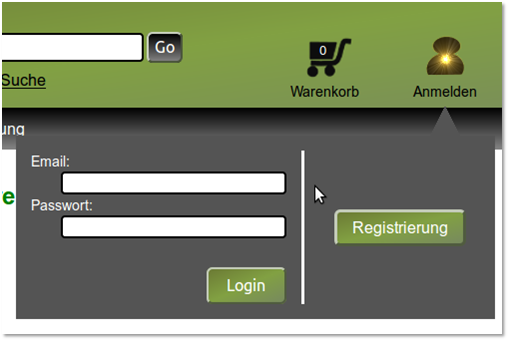
\includegraphics[width=75mm]{Bilder/Abbildung14_Loginbereich.png}
	\end{center}
	\caption{Flyout: Loginbereich}
\end{figure}

Die Besonderheit bei den Flyout des Webshops ist, dass es auch bei deaktivierten JavaScript funktioniert.  Das Flyout wurde mit den in CSS 2.0 eingeführten \glqq Kindselektor\grqq{} umgesetzt. Mit diesen \glqq Kindselektor\grqq{} ist es eingeschränlt möglich mit CSS eventbasiert zu programmieren. Um diese CSS-Funktion nutzen zu können muss aber folgende Bedingung erfüllt sein: Das Fenster, dass angezeigt werden soll muss ein Kindelement des Elements sein, welches das Ereignis auslöst. Die Syntax das \glqq Kindselektor\grqq{} sieht wie im \textit{Quellcode 3} zeigt aus. Am Anfang steht die Bedingung, die am Elternelement erfüllt sein muss. Beim Webshop wäre es die Bedingung, dass die Maus sich auf den Anmeldesymbol befinden soll. Diese Bedingung sieht in CSS geschrieben folgendermaßen aus: \glqq .accountCell:hover\grqq{}. Darauf folgt ein \glqq >\grqq{}-Zeichen. Dieses Zeichen legt fest, dass bei erfüllter Bedingung nicht die Style-Anweisung des Elternelements verändert werden soll, sondern eines Kindelementes. Nachfolgend wird das Kindelement angegeben, wo die Style-Anweisung geändert werden soll. Der letzte Teil der Style-Anweisung legt das neue Aussehen des Kindelements fest. Beim Webshop wird hier festgelegt, dass das Kindelement sichtbar werden soll. Ein Paar Zeilen vorher definiert eine Anweisung, dass das Kindelement unsichtbar sein soll. Bei gültiger Bedingung wird diese Anweisung wird einfach von der eben genannten Anweisung überschrieben.

\begin{center}
	\begin{lstinputlisting}[language=CSS, caption={Loginbereich: Umsetzung des Flyouts mit CSS 2.0}]
		{Quellcode/flylayout.css}
	\end{lstinputlisting}
\end{center}

\textbf{Kundenprofil ändern}\\
Hat sich eine Kunde angemeldet, so bietet der Webshop ihn die Möglichkeit die bestehenden Login-Daten und die persönlich Anschrift zu ändern. Erreicht können die Formulare zur Änderung der Daten über ein Flyout. Wenn der Kunde angemeldet ist wird das Flyout unter den Anmeldesymbol zu einen Menü geändert (siehe \textit{Abbildung 17}).
\begin{figure}[H]
	\begin{center}
			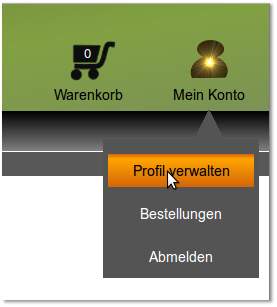
\includegraphics[width=55mm]{Bilder/Abbildung15_Menue_Profil_aendern.png}
	\end{center}
	\caption{Flyout: Kunde angemeldet}
\end{figure}

Bei diesem Menü muss der Eintrag \glqq Profil verwalten\grqq{} gewählt werden, um die bestehenden Login-Daten und die persönlich Anschrift ändern zu können. Nach der Anwahl des Eintrags bekommt der Kunde die in der \textit{Abbildung 18} gezeigte Seite zu sehen.
\begin{figure}[H]
	\begin{center}
			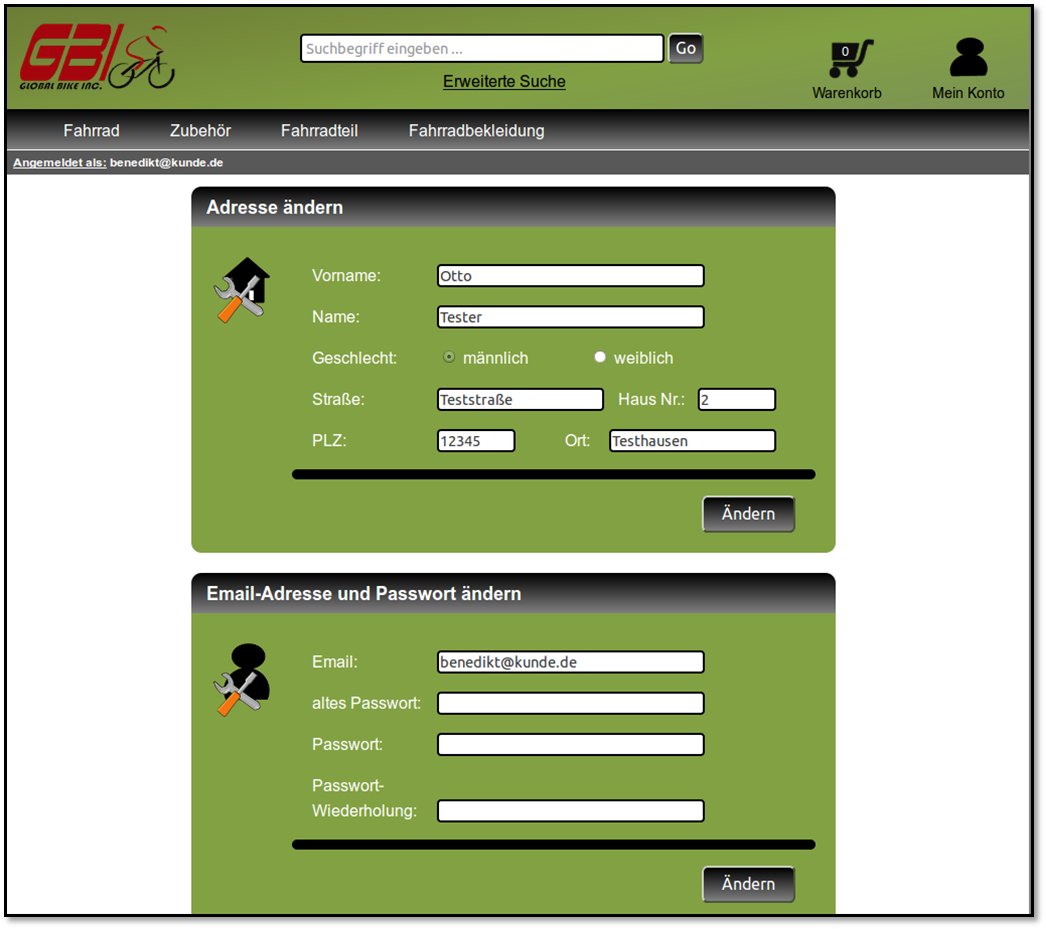
\includegraphics[width=130mm]{Bilder/formulare_profil_aendern.png}
	\end{center}
	\caption{Formulare Kundenprofil ändern}
\end{figure}
Die Änderung des Kundenprofils wurde mit Hilfe von zwei Formularen umgesetzt. Das erste Formular ändert die Anschrift des Kunden und das andere die Logindaten. Der Vorteil dieser zwei Formulare ist, dass somit die Seite übersichtlicher gestaltet ist und meist eh nur der Kunde die Adresse ändert, wenn er umgezogen ist. Häufiger wird es wahrscheinlich vorkommen, dass der Kunde das Loginpasswort ändert. Durch die Trennung der Adresse und der Logindaten werden bei Änderung des Passworts nur das neue Passwort und die Login-Email-Adresse an den Server übertragen und neu in die Datenbank geschrieben. Somit werden so wenig wie möglich unnötige Daten zum Server übertragen.\\
Technisch umgesetzt wurde der Vorgang wie beim Registrierungsvorgang. Wenn JavaScript aktiviert ist, überprüft die JavaScript-Funktion \glqq vorcheckEingabeEmailPasswort()\grqq{} oder \glqq vorcheckEingabeAdresse()\grqq{} browserseitig die Eingabe. Die aufgerufene Funktion ist abhängig von welchen Formular der Submit-Button geklickt wurde. Diese Funktionen sind in der Datei \glqq /Funktions/JS/ \\ vorcheck\_profil\_aendern.js\grqq{} vorzufinden. War die Überprüfung nicht erfolgtreich wird wieder eine Fehlermeldung auf den entsprechenden Formular ausgegeben. War die Überprüfung erfolgreich wird aus den bekannten Gründen diese nochmal auf dem Server durchgeführt. War die serverseitige Überprüfung erfolgreich, ruft die Funktionsdatei \glqq /Funktions/PHP/kunde\_aendern.php.inc\grqq{} die entsprechende Änderungsmethode der Klasse \glqq Kunde\grqq{} auf und übergibt der Methode als Parameter die Formulareingabe. Diese Methode ändert die entsprechenden Werte in der Datenbank mit Hilfe einer Update-SQL-Anweisung. Wurde die Änderung erfolgreich ausgeführt, wird der Kunde über eine Informationsbox darüber informiert.


%Arbeitspaket von Herrn Dück
\newpage
\subsection{Arbeitspaket von Herrn Dück$^4$}

Dieser Abschnitt beschreibt, wie Herr Dück die ihm zugeteilten Arbeitspakete bearbeitet und gelöst hat. Darunter fällt die Erstellung einer CSS-Datei für mobile Systeme, die Bewertung von Artikeln sowie die Gestaltung der Bestätigungs-E-Mail.


\subsubsection{Arbeitspaket 2: Die CSS-Datei für die Darstellung auf mobilen Geräten}

\textbf{Warum eine CSS-Datei für mobile Geräte?}
\\
Der Grund für eine zweite CSS ist der, dass auch auf Smartphones und Tablets die Homepage der GBI eine einfache und benutzerfreundliche Struktur haben soll. Ohne diese wird die Website so klein dargestellt, dass die gesamte Breite auf dem mobilen Gerät dargestellt wird.

\begin{figure}[H]
\begin{center}
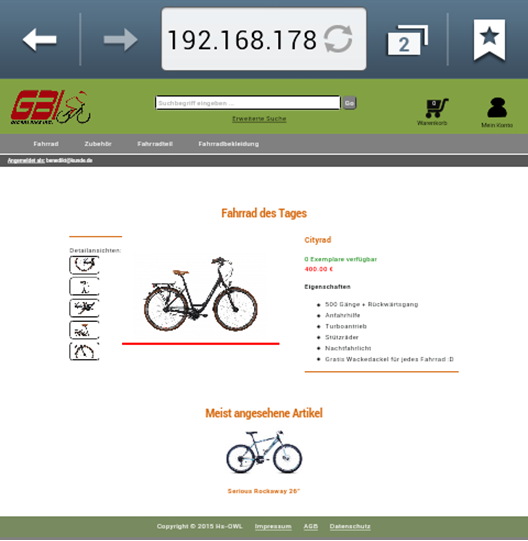
\includegraphics[width=12cm]{Bilder/Michael_Abbildung1-DarstellungDerWebsiteOhneMobileCSS.png}
\end{center}
\caption{Darstellung der Website ohne mobile CSS}
\end{figure}

Mit Tablets wird man damit nicht so große Probleme haben, dennoch muss auch für Tablets das Layout geändert werden. 
Mobile Geräte werden nicht mit einer externen Maus bedient sondern durch eine Touch-Funktion. Das verhindert die Darstellung von Dropdown-Menüs oder Popups durch die CSS-Formatierung ‚hover‘. Dieses Problem wird gelöst, in dem zusätzliche Seiten geschrieben werden, die dann das Dropdown-Menü und Popups ersetzen sollen.

\newpage
\textbf{Layoutgestaltung:}
\\
Zu Beginn der Bearbeitung dieses Paketes musste ein Design der mobilen Ansicht festgelegt werden. Angelehnt an den meisten Webseiten sollte auch hier ein verstecktes Menü eingebaut werden. Bei Klick auf einen Button fährt das Menü vertikal aus bzw. ein. Sowohl die Menüpunkte als auch die Funktionen, die im Header der Website sind, sollten in dieses Dropdown-Menü gelagert werden. Darunter fällt die Suchfunktion, der Zugriff auf den Warenkorb und der Login- bzw. Kontobereich. Der Header wird dementsprechend kleiner. Er enthält nur den Menü-Button und das Logo der GBI.
Formatierungen und Farben wurden größtenteils von der CSS-Datei für Desktop-Geräte übernommen. 
Der Designentwurf für mobile Endgeräte sieht folgendermaßen aus:

	
\begin{figure}[H]
\begin{center}
    \subfigure[Ohne Dropdown-Menü]{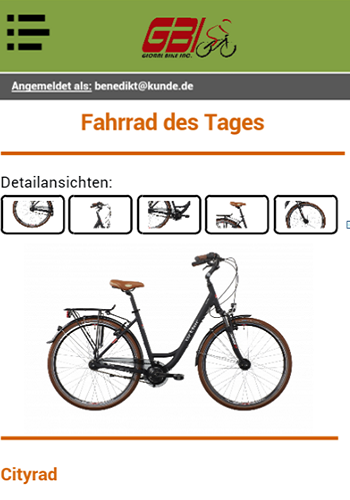
\includegraphics[height=10cm]{Bilder/Michael_Abbildung2-Desingentwurf.png}}
    \subfigure[Mit Dropdown-Menü]{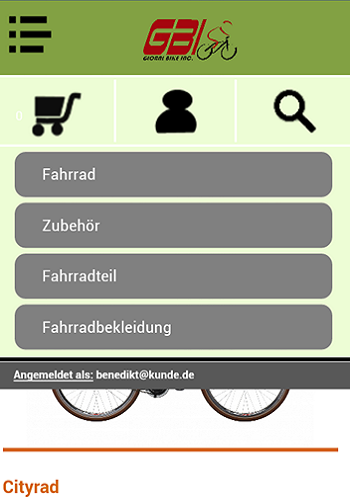
\includegraphics[height=10cm]{Bilder/Michael_Abbildung3-DesingentwurfMitDropDownMenue.png}}
\caption{Designentwurf}
\end{center}
\end{figure}

\textbf{Unterscheidung zwischen Desktop- und mobilen System:}
\\
Zunächst musste die Website beim Öffnen zwischen einen Desktop-System und einem mobilen Gerät unterscheiden können. Dies wird mit folgender Methode gelöst.
\newpage
\begin{center}
	\begin{lstinputlisting}[language=PHP, caption={Unterscheidung Desktop und mobiles Gerät}]
		{Quellcode/Michael-Quellcode1.php}
	\end{lstinputlisting}
\end{center}

Wenn die Methode ‚check\_mobile()‘ den Wert ‚false‘ ausgibt, handelt es sich um Desktop-System. Andern falls ist das Endgerät ein mobiles und zu der schon vorhandenen ‚style.css‘ wird die neue ‚mobile.css‘ importiert. Alle Änderungen, die notwendig für die Darstellung auf einem mobilen Gerät sind, werden hier gespeichert und überschreiben ggf. die Formatierungen in der ‚style.css‘.

\textit{Anpassen der Größen:}
\\
Es ist klar, dass die Website, so wie sie  vom ursprünglichen Desktop-Layout erzeugt wird, auf einem Smartphone viel zu klein dargestellt wird, das heißt die komplette Breite der Seite ist im Bild. Um das zu beheben, benötigt es nur eine Zeile in der ‚index.php‘.

\begin{center}
	\begin{lstinputlisting}[language=PHP, caption={Auszug aus der Index-Datei}]
		{Quellcode/Michael-Quellcode2.php}
	\end{lstinputlisting}
\end{center}

Mit diesem Ausdruck wird die Seite auf angenehme Größe heran gezoomt und kann nicht von Benutzer skaliert werden. 
Um das Benutzen der Website praktischer zu gestalten, sollte die Website auf einem mobilen Gerät nur in der vertikalen scrollbar sein. Das gilt sowohl für Handys als auch für Tablets. Im Grunde heißt das, dass die Breite der Website an die Breite des mobilen Gerätes angepasst werden muss. Da in der ‚style.css‘ viel mit Pixel-Breiten gearbeitet wird, bedeutet das, dass alle entsprechenden Elemente umformatiert werden müssen.
Zudem wurden außer Größen auch Anordnungen von Elementen und Farben geändert. Der Grund hierfür ist einfach, das die Website an einigen Stellen zu starke Farben hat und das evtl. unangenehm für den Benutzer werden kann. 



\begin{figure}[H]
\begin{center}
    \subfigure[]{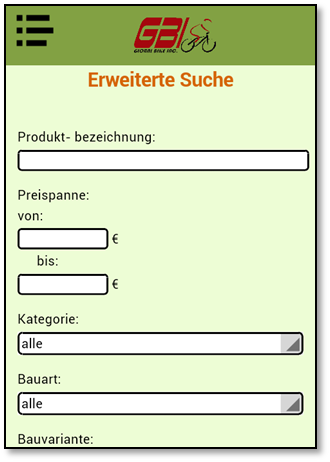
\includegraphics[height=8cm]{Bilder/Michael_Abbildung4-FarbaenderungenFuerBessereLesbarkeit1.png}}
    \subfigure[]{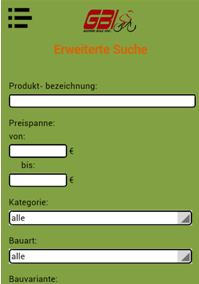
\includegraphics[height=8cm]{Bilder/Michael_Abbildung4-FarbaenderungenFuerBessereLesbarkeit2.png}}
\caption{Farbänderungen für bessere Lesbarkeit}
\end{center}
\end{figure}
\textbf{Menü}
\\
Ein großer Punkt bei der Gestaltung von mobilfähigen Websites ist das Menü. Das Menü kann auf einem Smartphone meist nicht so dargestellt werden, wie es auf der Desktop-Seite der Fall ist. Dort sind alle Menüpunkte in einer Reihe und dafür fehlt der Platz auf mobilen Geräten. Wenn die Menüpunkte untereinander angeordnet werden, ist der Header der Website zu großflächig. Es ist kaum was von dem Inhalt der Seite zu sehen. Aus diesem Grund ist ein Dropdown-Menü genau das richtige. So kann per Druck auf einen Button das Menü aus-, beziehungsweise eingefahren werden. Um den Platz noch sinnvoller zu nutzen, werden die drei Headerfunktionen, die Suche, der Warenkorb und die Kontofunktion, ebenfalls in das Dropdown-Menü versetzt.

\begin{figure}[H]
\begin{center}
    \subfigure[Das Dropdown-Menü]{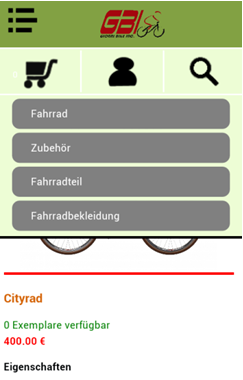
\includegraphics[width=5cm]{Bilder/Michael_Abbildung5-DasDropDownMenue.png}}
    \subfigure[Header mit fester Position]{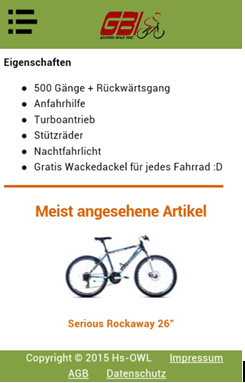
\includegraphics[width=5cm]{Bilder/Michael_Abbildung6-HeaderMitFesterPosition.png}}
\caption{Dropdown-Menü und Header}
\end{center}
\end{figure}

Der Header ist auf den Parameter ‚position: fixed‘ eingestellt, das heißt er hat eine festgesetzte Position und verändert sich nicht beim Scrollen der Seite. Das biete den Vorteil, dass das Menü jederzeit sichtbar und schnell erreichbar ist.
\\ \\
\textbf{Neue Seiten:}
\\
Im Laufe der Entwicklung der mobilen CSS wurden mehrere neue Seiten geschrieben. Das liegt daran, dass Funktionen, die auf dem Desktop-System recht praktisch sind, auf mobilen Geräten eher stören. Dazu zählen alle Popups als auch das Untermenü, welches erscheint, wenn man mit der Maus über den Menüpunkt ‚Fahrrad‘ geht. Um trotzdem nicht eingeschränkt zu sein, müssen folgende drei Seiten zusätzlich geschrieben werden:
\begin{enumerate}
\item Die Übersicht der Fahrradkategorien 
\item Eine Login-Seite
\item Eine Übersicht der Kontofunktionen
\end{enumerate}
Die Übersicht der Fahrradkategorien:
\\
Die Übersicht ist tatsächlich nur eine Auflistung aller Fahrradkategorien. Diese erreicht man, wenn der Menüpunkt ‚Fahrrad‘ geklickt wird. 
\\ \\
Eine Login-Seite
\\
Da Popups auf mobilen Geräten nicht angezeigt werden, gibt es sonst keine Möglichkeit sich anzumelden. Deswegen musste eine separate Seite geschrieben werden, auf die man gelangt, wenn man im Menü den Login-Button betätigt. Die Login-Seite bietet ebenfalls eine Weiterleitung zu der Registrierungs-Seite.

\begin{figure}[H]
\begin{center}
    \subfigure[Auflistung der Fahrradkategorien]{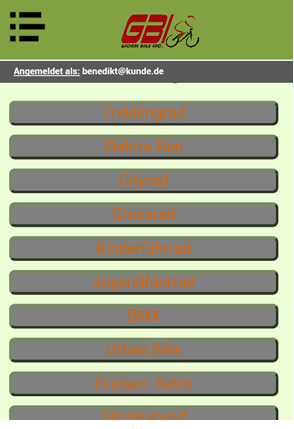
\includegraphics[height=8cm]{Bilder/Michael_Abbildung7-AuflistungDerFahrradkategorien.png}}
    \subfigure[Die Login-Seite]{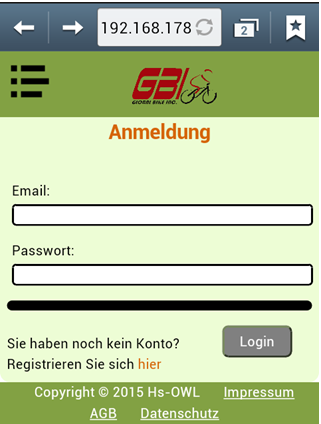
\includegraphics[height=8cm]{Bilder/Michael_Abbildung8-DieLogin-Seite.png}}
\caption{Auflistung der Fahrradkategorien und die Login-Seite}
\end{center}
\end{figure}

Eine Übersicht der Kontofunktionen
\\
Wie im vorherigen Punkt gibt es auch hier keine Möglichkeit, ohne Popup auf die Kontofunktionen zuzugreifen. Die neue Seite ‚(Name der Seite)‘ zeigt eine Übersicht dieser und kann durch Druck auf den Konto-Button erreicht werden.

\begin{figure}[H]
\begin{center}
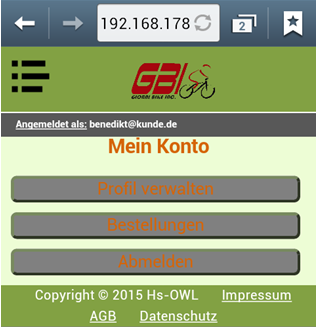
\includegraphics[height=8cm]{Bilder/Michael_Abbildung9-UebersichtDerKontofunktionen.png}
\end{center}
\caption{Übersicht der Kontofunktionen}
\end{figure}

\newpage
\textbf{Probleme/Hindernisse:}
\\
Ein Problem bei der Bearbeitung dieses Arbeitspaketes war die stetige Veränderung der Website, sowohl der PHP-Seiten als auch der CSS-Dateien. Dadurch wurde das Erstellen einer CSS-Datei für mobile Geräte zu einer Langzeitaufgabe, da immer wieder Teile geändert und angepasst werden mussten. 


\subsubsection{Arbeitspaket 11: Die Bewertungsfunktion von Artikeln}

Die Bewertung ist in einem Webshop eine große Hilfe bei der Findung guter Produkte. Deshalb soll diese Funktion in GBI-Webshop auch nicht fehlen. 
In diesem Abschnitt wird alles rund um die Bewertung von Produkten beschrieben. Dabei wird auf das Ansehen und auf das Verfassen einer solchen eingegangen.
\\ \\
Bewertung Popup
\\
Um sofort für jeden ersichtlich zu machen, wie ein Artikel bewertet wurde, befindet sich in der Artikelbeschreibung ein Feld mit der Durchschnittlichen Sternebewertung und dahinter eine Angabe, wie viele Bewertungen abgegeben wurden. So kann der Benutzer von vornherein sehen, ob dieser Artikel sich lohnt oder nicht. Will man genau wissen, wie die Aufteilung der Bewertungen auf die Sterne ist, bietet das Feld ein Popupfenster, welches erscheint, wenn man mit der Maus darüber fährt. Zusätzlich befindet sich in diesem Popup ein Link, über den man zu allen Rezensionen dieses Artikels weitergeleitet wird.

\begin{figure}[H]
\begin{center}
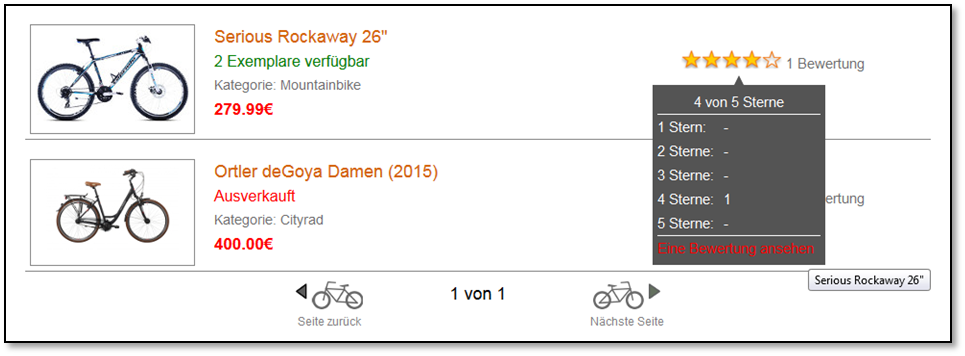
\includegraphics[width=12cm]{Bilder/Michael_Abbildung10-BewertungPopup.png}
\end{center}
\caption{Bewertung Popup}
\end{figure}

Einen Artikel bewerten
\\
Um selber eine Rezension zu diesem Artikel zu verfassen, befindet sich auf der Artikelseite der Link „Artikel bewerten“, über den man zu der Bewertungsseite gelangt. 
. Voraussetzung um eine Bewertung abgeben zu können, ist sich zuvor angemeldet zu haben. Ist das nicht der Fall, soll auf die Login-Seite weitergeleitet werden mit einem Hinweis sich anzumelden.

\begin{figure}[H]
\begin{center}
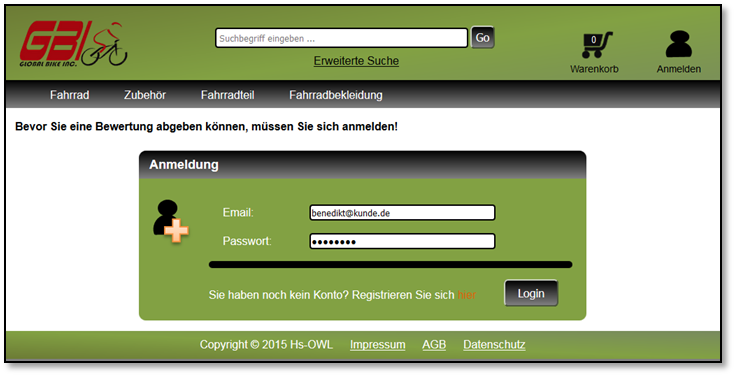
\includegraphics[width=12cm]{Bilder/Michael_Abbildung11-ArtikelBewertenOhneAnmeldung.png}
\end{center}
\caption{Artikel bewerten ohne Anmeldung}
\end{figure}

Ist man im System angemeldet, ist man berechtigt eine Bewertung zu verfassen.
Die Idee der Bewertungsfunktion ist angelehnt an die von Amazon. Der Benutzer muss drei Angaben machen, bevor die Bewertung abgegeben werden kann: Eine Sternbewertung, eine Überschrift und schließlich ein Text bzw. Kommentar. 

\begin{figure}[H]
\begin{center}
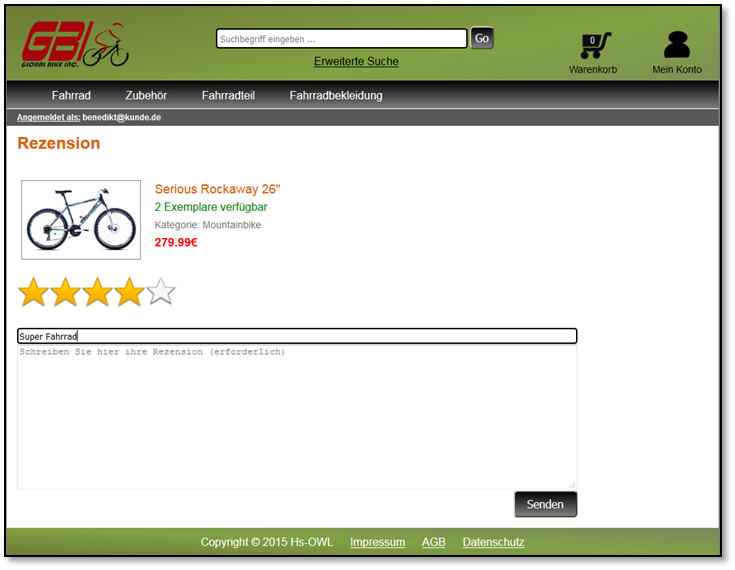
\includegraphics[width=12cm]{Bilder/Michael_Abbildung12-ArtikelBewertenMitAnmeldung.png}
\end{center}
\caption{Artikel bewerten mit Anmeldung}
\end{figure}

\newpage
Wird der Submit-Button geklickt, wird, wie auch bei der Suche oder Registrierung, über JavaScript überprüft, ob die Eingabe gültig ist. Dabei kommt es nicht auf den Inhalt des Geschriebenen an, sondern einfach nur dass alle Felder ausgefüllt sind. Sind alle Angaben gemacht worden, werden die Daten in die Datenbank geladen. Dazu wird die dafür zuständige Methode in der Klasse „Kommentar“ aufgerufen. Es wird sowohl die Produkt-ID als auch die Kunden-ID gespeichert. Das ermöglicht es, alle Bewertungen eines Produktes anzeigen zu lassen, als auch alle Bewertungen eines Kunden. Wenn ein Benutzer einen Artikel bewerten will, welcher schon zuvor von ihm bewertet wurde, wird seine ursprüngliche Bewertung angezeigt. Diese kann er dann nach Belieben ändern.
\\
Der Menüpunkt „Meine Rezensionen“
\\
Dem Benutzer soll es ermöglicht werden, all seine Rezensionen zu verwalten. Dazu wird in dem Menü zur Übersicht der Kontofunktionen ein neuer Menüpunkt erstellt: Meine Rezensionen. 

%\begin{figure}[H]
%\begin{center}
%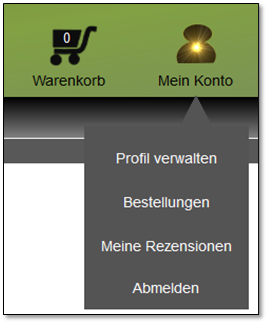
\includegraphics[width=4cm]{Bilder/Michael_Abbildung13-ZusaetzlicherMenuepunkt.png}
%\end{center}
%\caption{Zusätzlicher Menüpunkt}
%\end{figure}

Über diesen Button gelangt der Benutzer auf eine Seite all seiner Rezensionen und kann diese dort ändern oder löschen.

\begin{figure}[H]
\begin{center}
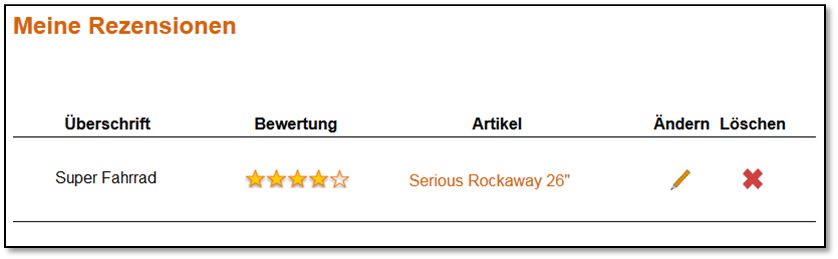
\includegraphics[width=12cm]{Bilder/Michael_Abbildung14-AnzeigeAllerRezensionenEinesBenutzers.png}
\end{center}
\caption{Anzeige aller Rezensionen eines Benutzers}
\end{figure}

\newpage

\subsubsection{Arbeitspaket 12: Die Gestaltung einer Bestätigungs-Email}

Wenn sich ein neuer Benutzer auf der Webseite registriert hat, wird, wie es bei den meisten Online-Shops der Fall ist, eine Bestätigungsmail an die E-Mail-Adresse gesendet, die bei der Registrierung angegeben wird. Dieses Verfahren ist notwendig, um die Korrektheit der E-Mail zu bestätigen. 
Solange die E-Mail vom Benutzer nicht bestätigt wurde, kann der Benutzer sich nicht im GBI-Webshop einloggen. Die Tabelle „kunde“ in der Datenbank enthält eine Spalte „aktiviert“, in die der Status steht. Sobald der Benutzer die E-Mail bestätigt, wird der Kunde aktiviert und kann sich nun im Webshop anmelden.
\\
Vorgehen:
\\
Die E-Mail wird versandt, nachdem die Eingabe bei der Registrierung auf dessen Gültigkeit überprüft worden ist und der Kunde zur Datenbank hinzugefügt wurde. 

%\begin{figure}[H]
%\begin{center}
%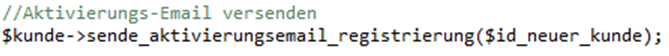
\includegraphics[width=12cm]{Bilder/Michael_Quellcode1.png}
%\end{center}
%\caption{IN QUELLCODE UMWANDELN Klasse Kunde ab Zeile 484!!!}
%\end{figure}

\begin{center}
	\begin{lstinputlisting}[language=PHP, caption={Aktivierungs-E-Mail versenden}]
		{Quellcode/Michael-Quellcode3.php}
	\end{lstinputlisting}
\end{center}

Die Methode \glqq sende\_aktivierungsmail\_registrierung\grqq{} der Klasse \glqq{Kunde}\grqq{} wird aufgerufen. In dieser Methode wird eine Verbindung zu der Datenbank hergestellt, um die Daten des Kunden auszulesen.  Dies ist erforderlich um die E-Mail kundenspezifischer zu gestalten.
Weiter wird der Anredesatz und die E-Mail-Nachricht verfasst.

%\begin{figure}[H]
%\begin{center}
%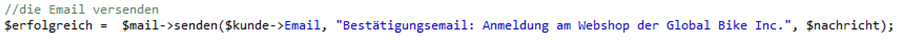
\includegraphics[width=12cm]{Bilder/Michael_Quellcode2.png}
%\end{center}
%\caption{IN QUELLCODE UMWANDELN!!!}
%\end{figure}

\begin{center}
	\begin{lstinputlisting}[language=PHP, caption={Die E-Mail versenden}]
		{Quellcode/Michael-Quellcode4.php}
	\end{lstinputlisting}
\end{center}

\newpage
Anschließend muss die E-Mail nur noch versandt werden.

%\begin{figure}[H]
%\begin{center}
%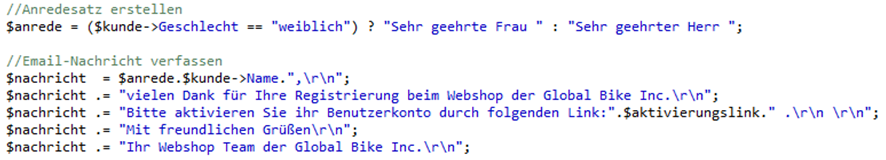
\includegraphics[width=12cm]{Bilder/Michael_Quellcode3.png}
%\end{center}
%\caption{IN QUELLCODE UMWANDELN!!!}
%\end{figure}

\begin{center}
	\begin{lstinputlisting}[language=PHP, caption={Anredesatz erstellen und E-Mail Nachricht verfassen}]
		{Quellcode/Michael-Quellcode5.php}
	\end{lstinputlisting}
\end{center}

Um den Kunden zu aktivieren, befinden sich in der gleichen Klasse die Methode \\
\glqq{aktiviere\_Kunde\_durch\_aktivierungs\_code}\grqq{}. 

%Webshopsicherheit
\section{Sicherheit}
Zum Schutz des Webshop vor Angriffen wurden mehrere Sicherheitsmechanismen in die Seite eingebaut. Dieser Abschnitt erläutert welche Sicherheitsmechanismen verbaut wurden und warum diese verbaut worden sind.

\subsection{\glqq .htaccess\grqq{}-Datei}
Als eine mögliche Schwachstelle sah das Projektteam an, dass PHP-Dateien direkt über die Adressenleiste im Browser aufgerufen werden können. Es könnte zum Beispiel somit ein Benutzer durch direktes aufrufen einer Datei, versuchen den Passwortschutz der Webseite zu umgehen. Dieser Benutzer wäre dann vielleicht in der Lage Produkte zu kaufen ohne registriert zu sein. Diese Schwachstelle wurde gelöst indem nur die Index-Datei direkt aufgerufen werden kann. Die Index-Datei erhielt somit als einzige Datei die Endung \glqq *.php\grqq{}. Alle anderen PHP-Skripte bekamen die Dateiendung \glqq *.php.inc\grqq{}. In einer sogenannten \glqq .htaccess\grqq{}-Datei wurde danach festgelegt, dass von Browser aus die \glqq *.php.inc\grqq{}-Dateien nicht geöffnet werden können. Um die Skripte mit \glqq *.php.inc\grqq{}-Endung ausführen zu können, werden diese zum vorgesehenen Zeitpunkt in die Index-Datei inkludiert. Die ganze Webseite wird somit komplett durch die Index-Datei abarbeitet.\\
Des Weiteren wurde mit der \glqq .htaccess\grqq{}-Datei festgelegt, dass der Browser nicht alle Dateien eines Verzeichnisses auflisten darf. Hiermit sollte sichergestellt werden, dass der unerwünschte Benutzer nicht die Ordnerstruktur der Webseite ermitteln kann.

\subsection{Schutz vor: Cross-Site-Scripting (XSS) und SQL Injection}
Als eine weitere Schwachstelle wurde Cross-Site-Scripting (XSS) und SQL Injection angesehen. Bei SQL-Injection versucht eine Angreifer Schadcode in die Datenbank einzuspielen. Hierzu nutzt der Angreifer den Aufbau einer SQL-Anweisung aus. Bei einer SQL-Anweisung werden die zu übergebenen Werte zwischen zwei Hochkomma geschrieben. Der Angreifer schreibt dann in das Textfeld, wovon die Werte in die Datenbank übernommen werden sollen, ein Hochkomma und ein Semikolon. Dadurch geht die SQL-Datenbank davon aus, dass die Datenbankanweisung schon an der Stelle zu Ende ist. In SQL können durch Semikolons mehrere Anweisungen hintereinander geschrieben werden. Somit wäre es möglich, dass der Angreifer nun zum Beispiel eine Anweisung in das Textfeld schreibt, dass die Datenbank gelöscht werden soll und alle Daten weg sind. Zum Schutz vor dieser Situation bietet das \glqq MYSQLi\grqq{}-API die Methode \glqq real\_escape\_string()\grqq{}. Die gerade genannte Methode \glqq escaped\grqq{} alle Hochkomma, sodass diese nicht mehr der SQL-Anweisung schaden können. Cross-Site-Scripting beschreibt einen ähnlichen Vorfall. Hier tippt der Angreifer einen JavaScript in die Textfelder ein. Dieses mal ist von den Angriff der Browser betroffen. Soll nun zu einen späteren Zeitpunkt die Texteingabe auf der Webseite ausgegeben werden, so wird im Browser der JavaScript ausgeführt. Zum Schutz vor einer solchen Situation bietet PHP die Funktion \glqq htmlspecialchars\grqq{}. Mit der Funktion \glqq htmlspecialchars\grqq{} werden Steuerzeichen von HTML ( \&, ", <, >) durch die HTML-Ersatzschreibweise ersetzt. Die Ersatzschreibweise hat zu folge, dass der JavaScript nicht mehr ausgeführt wird. Der \glqq Schadcode\grqq{} wird nun einfach als Text auf der Webseite ausgegeben. 

%Fazit
%=============================================
%Muss nochmal ein bisschen überarbeitet werden
%=============================================

\section{Fazit}

Nachfolgend soll noch einmal kurz darauf eingegangen werden, wie der Verlauf des Projektes zu beurteilen ist. Dabei wird sich auch zu der Motivation innerhalb der Gruppe und der Zusammenarbeit mit anderen Gruppen geäußert.


\subsection{Motivation innerhalb der Gruppe}

Die Motivation innerhalb der Gruppe war unterschiedlich. Während sich die Gruppenmitglieder Herr Schnürer und Herr Brüntrup stets bemühten die Arbeit an den Webshop voranzutreiben, lies die Motivation der beiden Gruppenmitglieder Herr Gregarek und Herr Dück etwas zu wünschen übrig.  Bei letzteren war die Teilnahme am Projekt nicht immer vollständig vorhanden, was sich auch darin wiederspiegelt, das Herr Gregarek und Herr Dück nicht zu allen Treffen erschienen sind.

\subsection{Zusammenarbeit mit anderen Gruppen}
Die Zusammenarbeit mit anderen Gruppen gestaltete sich durchgehend positiv. Die wichtigsten Schnittstellen waren hierbei die Server-, SAP- sowie die APP-Gruppe. Zu jeder Gruppe herrschte ein reger Austausch, sodass entsprechende Schnittstellen leicht implementiert werden konnten.


\subsection{Verlauf des Projektes}

Abgesehen von kleinen Differenzen innerhalb der Gruppe hinsichtlich der Motivation, konnte das Projekt rechtzeitig vollendet werden. Durch der unterschiedlichen Arbeitsleistung bedingt, mussten jedoch einzelne Arbeitspakete neu verteilt oder mangels der nötigen Zeit gekürzt werden. Da die wichtigsten Funktionen, die der Webshop gemäß der Aufgabenerstellung erfüllen soll erfolgreich implementiert worden sind, lässt sich der Verlauf des Projektes abschließend durchaus positiv beurteilen.

%Quellenverzeichnis
\newpage
\section{Autorenverzeichnis}
\begin{itemize}
	\item[$^1$] Herr Brüntrup
	\item[$^2$] Herr Schnürer
	\item[$^3$] Herr Gregarek
	\item[$^4$] Herr Dück
\end{itemize}



\section{Quellenverzeichnis}

\subsection*{Vorlesungen}
\begin{itemize}
	\item Websdesign - Prof. Dr. rer. nat. Stefan Wolf
	\item Datenbanken - Prof. Dr.-Ing. Klaus Maas  
\end{itemize}

\subsection*{Literatur}
\begin{itemize}
	\item \textsc{Asmuth, M.} (2009): \textit{Online-Projekte mit PHP und MySQL} -  3.Auflage - \\ Bildungsverlag EINS
	\item \textsc{Reese, G. \&  Schulten, L.} (2006): \textit{MySQL - kurz $\&$ gut} -  2.Auflage - O'REILLY
\end{itemize}

\subsection*{Onlinequellen}
\begin{itemize}
	\item http://php.net (Stand: 29. August 2015)
	\item http://selfhtml.org/ (Stand: 29. August 2015)
	\item http://www.w3schools.com (Stand: 29. August 2015)
	\item http://www.css4you.de/wscss/css03.html (Stand: 29.August 2015)
\end{itemize}



\end{document}